\documentclass[a4paper, 12pt, fleqn]{article}
\usepackage{custom}
\usepackage{titlepage}
\usepackage[bottom]{footmisc}
\usepackage{wrapfig}

%============STYLE PROPERTIES============
\setlength{\parindent}{0pt}

\graphicspath{{../}}

%============PAGE PROPERTIES=============
\newcommand{\revisiondate}{\today}
\newcommand{\documenttitle}{CM\_PrivLaw} % used for title in title and subtitle pages
\newcommand{\authors}{Diego Bienz \& Michael Blättler} %used for title page only
\newcommand{\subtitle}{Zusammenfassung} % used for title and subtitle pages
\newcommand{\documentdesc}{Zusammenfassung}
\newcommand{\ort}{Hochschule Luzern Technik \& Architektur, Horw}

%============REF-COMMANDS================
\newcommand{\secref}[1]{\hyperref[{#1}]{\autoref*{#1}}}
\providecommand{\tightlist}{\setlength{\itemsep}{0pt}\setlength{\parskip}{0pt}}

\begin{document}
	\begin{titlepage}
		\appendixGM
		\thispagestyle{empty}
	\end{titlepage}

	\tableofcontents

	\section{Einführung ins Recht und dessen Privacy-Aspekte}

\subsection{Recht im technischen Umfeld}

Das Recht legt auch oft einen \textbf{Rahmen} des rechtlich Verlangten
fest (was ist maximal zulässig, was wird minimal verlangt?). Also
\textbf{Aufklärung \& Festlegung von Standards und Verpflichtungen und
Verantwortlichkeiten}. Die Standards werden zwar nicht vom Gesetz
festgelegt, aber es wird darauf verwiesen.

\emph{ABER: Standards/Best Practices klären oft nicht ausreichend alle
rechtlichen Fragen}

\subsection{Recht als ``Risk Management''}

Risiken müssen nicht nur technisch und organisatorisch behandelt werden,
sondern es müssen auch \textbf{rechtliche Massnahmen} getroffen werden.
\textbf{Juristische Probleme können technisch behandelt werden} und
umgekehrt können technische Probleme juristisch gelöst werden.

\emph{Rechtliche Unterstützung möglichst früh im Projekt einschalten
Das Management ist dabei verantwortlich für die Einhaltung von Vorschriften
zu organisieren und zu kontrollieren.}

\subsection{Weshalb Privacy \& Datenschutz?}

\textbf{Personenbezogene Daten in den falschen Händen können eine Person
in vielfältiger Form gefährden \& verletzen}. Vertraulichkeit und das
\textbf{``Recht auf Vergessen''} ist elementar. Inhaber von grossen
Mengen an personenbezogenen Daten haben eine machtvolle Stellung ohne
Kontrolle. Einer der Hauptaufgaben eines Staates ist es, seine Bürger zu
beschützen. Doch wie kann er das bzgl. Missbrauch von Personendaten?\\
Zusätzlich haben personenbezogene Daten einen gewissen finanziellen Wert.
Wer ist berechtigt, diese Daten zu nutzen und zu verwerten?
Unsere Daten werden einmal verkauft, aber ökonomisch fortgesetzt genutzt.

\mbox{}\\
\emph{Die Weitergabe von persönlichen Daten in einem Unternehmen ist
auch eine Form von Mobbing und/oder schlechtem Management.}

\subsection{Zentrale (Obligationenrechtliche) Frage}

\begin{enumerate}
\def\labelenumi{\arabic{enumi})}
\tightlist
\item \textbf{WER} will
\item von \textbf{WEM}
\item \textbf{WAS}
\item \textbf{WORAUS}?
\end{enumerate}

\emph{Obligationenrechtlich = Fragen nach Rechtsansprüchen, z.B. aus Vertrag,
unerlaubter Handlung oder ungerechtfertigter Bereicherung.}

\subsection{Site, Moral und Recht}

Rechtliche Verbindlichkeit ist für alle einzufordern (\textbf{grösster
gemeinsamer Nenner} einer vielfältigen Gemeinschaft)


\subsection{Die Juristische Argumentation (!)}

Eine juristische Argumentation sieht immer so aus, dass man eine
Behauptung aufstellt und diese anschliessend begründet. Die Begründung
beruht auf einem Beweis oder einem Gesetzesartikel.

\mbox{}\\
\textbf{Behauptung} wird durch Grundlage (\textbf{Gesetzesartikel}) und
notwendigen \textbf{Beweis} gestützt.\\
\\
\textit{oder}\\ 
\\
Gestützt auf Grundlage (\textbf{Gesetzesartikel}) und notwendigem
\textbf{Beweis} ergibt sich die \textbf{Schlussfolgerung}.


\subsection{Rechtsordnung unter verschiedenen Blickwinkeln}
%
\begin{itemize}
\tightlist
\item Rang (Verfassung, Gesetz, Verordnung)
\item erlassendem Gemeinwesen (Bundesrecht, kantonales- und
Gemeinderecht)
\item Rechtsquelle (geschriebenes Recht, Gewohnheitsrecht,
Gerichtspraxis (Gesetzesauslegung), ZGB)
\item Beteiligten Personen (Privatrecht, öffentliches Recht)
\end{itemize}


\subsection{Hierarchie des Rechts}

\begin{verbatim}
----------------
| Verfassung   |
----------------
       |
----------------
| Gesetze      |
----------------
       |
----------------
| Verordnungen |
----------------
\end{verbatim}

Verordnungen \textbf{sind keine} Verfügungen.\\
Beispiele für Verfügungen: Eine Hochschule besitzt die Verfügung,
Personen als Ingenieur auszuzeichnen.

\subsubsection{Bund/Kantone/Gemeinden}

Kantone stehen in der Gesetzgebungsmacht über dem Bund! Kantone aber
über den Gemeinden

\subsection{Privat- vs. öffentliches Recht}

\begin{description}
	\item[Privatrecht] Zwischen natürlichen bzw. juristischen Personen.\\
	Geprägt vom Grundsatz der \textbf{Koalitions- und Vertragsfreiheit}.
	\item[Öffentliches Recht] Zwischen Staat und natürlichen/juristischen
	Personen.\\
	\textbf{Legalitätsprinzip (Gewaltenkontrolle)}\index{Legalitätsprinzip}
	\index{Gewaltenkontrolle}:
	Der Staat darf nur handeln,
	wenn eine gesetzliche Grundlage besteht!
\end{description}

\subsection{Anwendbarkeit von ausländischem Recht}

\begin{itemize}
	\tightlist
	\item Nebst Völkerrecht, (bi-/multilateralen) internationalen Verträgen ist
	das IPRG (Gesetz über das internationale Privatrecht)\index{IPRG}
	``Hauptschnittstelle'' zwischen CH- und ausländischem Recht.
	\item IPRG regelt, wann welches Recht (CH oder Ausland) anwendbar ist und
	welche Richter zuständig sein sollen.
\end{itemize}

\subsection{Instanzenzug}

Zivil-, Verwaltungs- und Strafgerichte haben unterschiedliche
Verfahren. In allen Rechtsbereichen gibt es jedoch drei Instanzen:

\begin{enumerate}
	\tightlist
	\item Bezirksgericht
	\item Kantonsgericht
	\item Bundesgericht
\end{enumerate}

\subsection{Verschiedene Prozessverfahren und deren Eigenheiten}

\subsubsection{Zivilprozess}

\begin{itemize}
\tightlist
\item Prozesse müssen vor dem örtlich/sachlich \textbf{zuständigen} Gericht
  ausgetragen werden.
\item Ein \textbf{Gerichtskostenvorschuss} ist nötig, um ein Zivilverfahren
  einzuleiten. Der Vorschuss ist abhängig vom Streitwert.
\item Das Gericht sucht keine Beweise. Der \textbf{behauptete Anspruch muss
  bewiesen werden können}.
\item Wer verliert, muss die \textbf{Gerichtskosten sowie Parteikosten der
  andern Seite übernehmen}.
\item Wer einen Forderungsprozess gewinnt, hat das Geld \textbf{noch
  nicht}\ldots{}
\end{itemize}


\subsubsection{Strafverfahren}

\begin{itemize}
	\tightlist
	\item Geregelt im StGB \& StPO. Polizei unterliegt überwiegend
	kantonaler Hoheit.
	\item Für Antragsdelikte (bspw. Diebstahl, Ehrverletzung) gilt eine Frist 
	von \textbf{3 Monaten}!
	\item Staatsanwaltschaft leitet Untersuchung und muss \textbf{belastende \&
	entlastende} Aspekte sammeln.
	\item  Die Einsicht als Beteiligter ist Begrenzt. Durch das Einreichen einer
	\textbf{Privatstrafklageverfahren}\index{Privatstrafklageverfahren}
	bekommt man als Opfer erweitertes Einsichtsrecht.
	\item Der Staatsanwaltschaft stellt das Verfahren ein, straft mit max.
	6 Monaten Freiheitsstrafen und/oder 180 Tagessätze oder überweist den
	Fall zur Beurteilung an das Strafgericht.
	\item Als Verurteilter kann das Urteil auch an das Strafgericht
	weitergezogen werden.
\end{itemize}


\subsection{Verwaltungsverfahren}

\begin{itemize}
	\tightlist
	\item \textbf{Verfügungen} müssen immer durch die \textbf{richtige Behörde}
	im \textbf{richtigen Verfahren} und unter \textbf{Angabe der
	Rechtsmittels} dagegen erlassen werden. Fehlt eine dieser
	Voraussetzungen, ist die Verfügung nichtig!
	\item Wenn neue Tatsachen auftauchen, ist es möglich eine
	Wiedererwägung/Einsprache gegen die Verfügung zu erheben. -Gegen
	Verfügungen kann i.d.R. Beschwerde innert 10/20/30 Tagen geführt
	werden.
	\item Je nach Gesetzesgrundlage ist ein kantonales Obergericht oder das
	Bundesgericht höchste Instanz.
\end{itemize}

    \section{Grundzüge des Urheberrechts}

\subsection{Immaterialgüterrecht (Geistiges Eigentum)}
Schutz vor ungreifbaren (immateriellen) Gütern.\\
Die verschiedenen Bereiche des Immaterialgüterrecht sind:
\begin{itemize}
	\tightlist
	\item Urheberrechte (z.B. Rechte an Fotografien)
	\item Designrechte
	\item Patentrechte
	\item Markenrechte
\end{itemize}

\subsection{Schutzvoraussetzungen}
\label{sec:Urheberrecht-Schutzvoraussetzugen}

\begin{figure}[H]
	\centering
	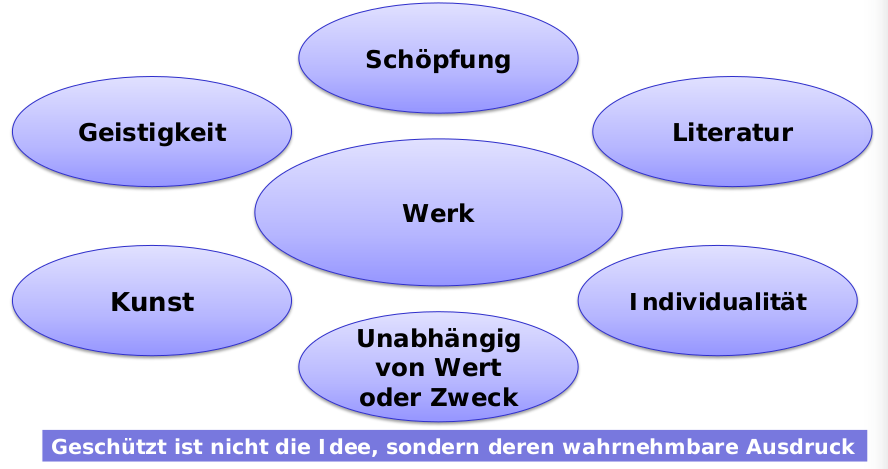
\includegraphics[width=0.6\textwidth]{figures/urheberrechtsSchutz.png}
	\caption{Was ist geschützt?}
\end{figure}

Folgende Werke zählen zum Immaterialgüterrecht:
\begin{enumerate}
\tightlist
\item Literarische, wissenschaftliche und andere Sprachwerke
\item Werke der Musik und der bildenden Kunst
\item Werke mit wissenschagtlichen oder technischem Inhalt
\item Computerprogramme
\item Werke der Baukunst
\item Fotographische, filmische oder visuelle Werke
\end{enumerate}

\textbf{Sonderfall: Werke zweiter Hand (Art. 3 URG}\\
Schöpfungen mit individuellem Charakter, die \textbf{unter Verwendung
bestehender Werke} so geschaffen werden, dass die verwendeten Werke in
ihrem individuelle Charakter erkennbar bleiben.

\subsection{Urheberschaft - Miturheberschaft}
\label{sec:Urheberrecht-UrheberschaftMiturheberschaft}

\textbf{Urheber} ist die \textbf{natürliche Person}, die das Werk
geschaffen hat (Art. 6 URG) --> \textbf{Schöpferprinzip}\index{Schöpferprinzip}.

Eine \textbf{Miturheberschaft} liegt vor, wenn mehrere Personen
gemeinsam, d.h. in \textbf{bewusster Zusammenarbeit} und nach einem
\textbf{gemeinsamen Konzept}, ein Werk schaffen. Dabei steht das
Urheberrecht allen gemeinsam zu (\textbf{Zustimmung aller Miturheber
nötig!})

\subsection{Abhängige Werkschöpfung}
\label{sec:Urheberrecht-AbhängigeWerkschöpfung}
Auch wenn ein Werk \textbf{im Rahmen eines Abhängigkeitsverhältnisses}
geschaffen wird, erwirbt der \textbf{Schöpfer originär} das
\textbf{Urheberrecht}. Nur für \textbf{Computerprogramme} kennt das URG
eine entsprechende Norm (Art. 17 URG). Diese gilt aber auch \textbf{nur}
für den \textbf{Arbeitsvertrag} und nicht für Auftrags- und
Werkvertragsverhältnisse.

\mbox{}\\
\emph{Arbeitgeber sollte sich im Arbeitsvertrag sämtliche Urheberrechte
abtreten zu lassen.}


\subsection{Urheberrechte}

\subsubsection{Urherberpersönlichkeitsrechte}
\label{sec:Urheberrecht-Urherberpersönlichkeitsrechte}
\textbf{Können nicht übertragen werden!}

\begin{itemize}
	\tightlist
	\item Recht auf Erstveröffentlichungen (Art. 9.2 URG)
	\item Recht auf Anerkennung der Urheberschaft (Art. 9.1 URG)
	\item Recht auf Werkintegrität (Art. 11 URG)
\end{itemize}

\subsubsection{Verwendungsrechte}
\textbf{Können übertragen werden! (e.g. im Arbeitsvertrag)}

\begin{itemize}
	\tightlist
	\item Vervielfältigungsrecht
	\item Verbreitungsrecht
	\item Recht auf öffentliche	Wahrnehmbarmachung
	\item Senderechte
	\item Weitersenderechte
	\item Vermieten von Computerprogrammen
	\item Bearbeitungsrecht
\end{itemize}

\subsection{Schutzvoraussetzungen und -dauer}

Der urheberrechtliche Schutz beginnt \textbf{ohne irgendeine Anmeldung}
in dem Moment, in dem ein Werk die Schutzvoraussetzungen erfüllt, d.h.
sobald die Grenze der Individualität überschritten wird (auch Entwürfe
sind geschützt).

Schutzdauer \textbf{70 Jahre nach dem Tod} des Urhebers (\textbf{50
Jahre} bei \textbf{PC-Programmen}). Wenn mehrere Urheber vorhanden sind,
dann beginnt diese Zeit, wenn der letzte ins Gras beisst.

\subsection{Schranken des Urheberrechtsschutzes}
\label{sec:Urheberrecht-Schranken}

Bei folgenden Anwendungen gilt das Urheberrecht nicht (Auswahl aus Art. 19 URG):

\begin{itemize}
	\tightlist
	\item Schulgebrauch
	\item Privatgebrauch
	\item Betriebsinterner Gebrauch
	\item Vorübergehende Vervielfältigung
	\item Archivierungs- und Sicherungsexemplare
	\item Entschlüsselung von PC-Programmen
	\item Zitate
\end{itemize}

\subsection{Urheberrecht im Internet}

\begin{itemize}
	\item \textbf{Vorsichtsmassnahmen}
	\begin{itemize}
		\item Bilder und Logos schützen
		\item Content mit Copyright versehen
		\item Dokumentierung der Alterspriorität (Fotos mit Datum)
		\item Nur Verkleinerungen ins Netz stellen
		\item Fotos mit unsichtbaren Metadaten versehen (z.B. Copyright)
		\item Banner eines Plagiaterkennungsdienstes auf Webseite aufschalten
	\end{itemize}
	\item \textbf{Rechtsschutzmassnahmen}
	\begin{itemize}
		\item Duplikate suchen
		\begin{itemize}
			\item Abklärung via web.archive.org
			\item Finderlohn-Aussetzung
		\end{itemize}
		\item Entfernungsaufforderung and Störer
		\item Abmahnung an Störer / Zustellung eines cease and desist letter
		\index{cease and desist letter}
		\item Internetprovider erforschen / Aufforderung an Provider zur
		Inhaltslöschung
		\item Suchmaschinenbetreibern anzeigen
	\end{itemize}
\end{itemize}

\subsection{Rechtsübergang und Rechte an Programmen}
\label{sec:Urheberrecht-Rechtsübergang}
\begin{itemize}
	\tightlist
	\item Die Verwendungsrechte an einem Werk sind unter Lebenden oder
	\textbf{von Todes wegen} vollständig auf Dritte \textbf{übertragbar}.
	\item Die Urheberpersönlichkeitsrechte sind unter Lebenden nicht
	übertragbar, von Todes wegen gehen sie jedoch auf die Erben über.
	(Art. 16.1 URG)
	\item Als einzige können Computerprogramme als Dienstwerke geschaffen
	werden, sofern der Urheber in einem Arbeitsverhältnis steht und dieses
	zu diesem Zweck (d.h. Schaffung von Computerprogrammen) besteht.
	(Art. 17 URG, vgl. Art. 332 OR)
\end{itemize}

\subsection{Rechtsschutz}

\begin{itemize}
	\item \textbf{Zivilrechtlicher Schutz}
	\begin{itemize}
		\item \textbf{Art. 61 - 66 URG}
		\begin{itemize}
			\item Feststellungsklage
			\item Leistungsklagen
			\item Einziehung im Zivilverfahren
			\item Vorsorgliche Massnahmen
			\item Veröffentlichung des Urteils
		\end{itemize}
		\item \textbf{Art. 41 und 97 OR}\\
		Schadensersatz und Genugtuung.
	\end{itemize}
	\item \textbf{Strafrechtlicher Schutz}
	\begin{itemize}
		\item \textbf{Art. 67 URG}
		\begin{itemize}
			\item Antragsdelikt
			\item Offizialdelikt bei Gewerbsmässigkeit\\
			Gefängnisstrafen bis zu 3 Jahren.
		\end{itemize}
		\item \textbf{Art. 68 URG}
		\item \textbf{Art. 69 - 73 URG} weitere Bestimmungen
		\item Ergänzend UWG und DSG beachten
	\end{itemize}
\end{itemize}

\subsection{Escrow-Agent}
Um die Leistung einer anderen Firma sicherzustellen, ist es möglich ein
sogenanntes \textbf{Escrow-Agreement} zu vereinbaren. Dabei wird der
Sourcecode einer Software einem \textbf{Escrow-Agent} gegeben, der diesen
unter Verschluss hält. Falls die Software nicht den abgemachten Leistungen
entspricht, hat man die Möglichkeit den Sourcecode beim Escrow-Agent
einzufordern um eine andere Firma mit der Weiterentwicklung zu beauftragen.
Das Agreement definiert die Regeln, wann der Sourcecode herausgegeben wird.

    \section{Privacy \& Datenschutz}

\subsection{Weshalb Privacy und Datenschutz}
Privatsphäre ist ein Menschenrecht. Alle modernen Demokratien schützen
diese! Im Grundsatz..

Um einen liberalen Lebensstil zu wahren, muss jeder Bürger selbst
entscheiden können \textbf{welche} Informationen er zur Verfügung stellt
und \textbf{wie} diese benutzt werden dürfen.


\subsection{Sphärentheorie}
Jeder entscheidet selbst, welche Daten/Information in welcher Sphäre
ist, weil jeder steht dazu was er macht.

\begin{figure}[H]
\centering
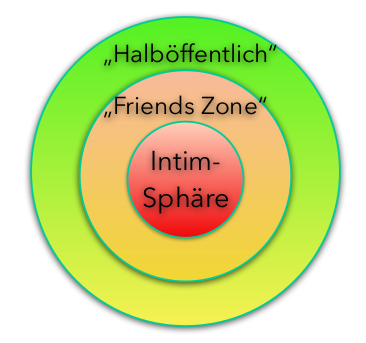
\includegraphics[width=.5\textwidth]{figures/sphaerentheorie.png}
\caption{Sphärentheorie}
\end{figure}

\textbf{Persönlichkeitsverletzung}:
\index{Persönlichkeitsverletzung}
Wenn Daten/Informationen von einer
Drittperson weitergegeben werden und somit ein Sphärenübertritt
stattfindet, spricht man von einer Persönlichkeitsverletzung.


\subsection{Schutz der Persönlichkeit}
\label{sec:Datenschutz-SchutzPersönlichkeit}

Ist im Art. 28 ZGB geregelt:\\
Wer in seiner Persönlichkeit \textbf{widerrechtlich} verletzt wird, kann zu
seinem Schutz gegen jeden, der in der Verletzung mitwirkt, das \textbf{Gericht}
anrufen.

\mbox{}\\
Eine Verletzung ist \textbf{widerrechtlich}, wenn sie nicht durch
\textbf{Einwilligung des Verletzten}, durch ein \textbf{überwiegend privates
oder öffentliches Interessen} oder durch \textbf{Gesetz} gerechtfertigt ist.


Dieses Gesetz stammt nicht vom Datenschutzgesetz, sondern vom
Zivilgesetzbuch.

Öffentliches Intresse besagt nicht, was die Öffentlichkeit
\textbf{interessiert} sondern was für die Öffentlichkeit
\textbf{relevant} ist.


\subsection{Datenschutz}
Als Datenschutz versteht man der Schutz der \textbf{Integrität} einer
Person vor Verletzungen Dritte.

Datenschutz ist\ldots{}

\begin{itemize}
	\tightlist
	\item Schutz der \textbf{informationellen Sebstbestimmung}
	\item Schutz der Persönlichkeit bei der Datenverarbeitung
	\item Schutz der Privatsphäre
	\item Schutz vor missbräuchlicher Datenverbreitung
\end{itemize}


\subsection{Gesetzliche Grundlagen}

\begin{itemize}
	\tightlist
	\item Schweizerische Bundesverfassung (Art. 13 BV)
	\item Bundesgesetz über den Datenschutz (DSG) und Verordnung dazu (VDSG)
	\item Zahlreiche datenschutzrechtliche Bestimmungen in anderen Gesetzen
	\item Kantonales und Gemeinderecht: zahlreiche Gesetze und Verordnungen
	\item International: Europäische Datenschutzrichtlinie bzw. -Grundverordnung
	(DSGVO/GDPR)
\end{itemize}

\subsection{Das schweizerische Datenschutzgesetz (DSG)}

\subsubsection{Geltungsbereich (Art. 2 DSG)}
\label{sec:Datenschutz-Geltungsbereich}

\begin{enumerate}
	\tightlist
	\item Dieses Gesetz gilt für das Bearbeiten von Daten \textbf{natürlicher
	und juristischer Personen} durch
	\begin{itemize}
		\tightlist
		\item private Personen;
		\item Bundesorgane.
	\end{itemize}
	\item Es ist nicht anwendbar auf:
	\begin{itemize}
		\tightlist
		\item Personendaten, die eine \textbf{natürliche Person ausschliesslich
		zum persönlichen Gebrauch bearbeitet und nicht an Aussenstehende bekannt
		gibt};
		\item Beratungen in den Eidgenössischen Räten und in den
		parlamentarischen Kommissionen;
		\item \textbf{hängige Zivilprozesse, Strafverfahren}, Verfahren der
		internationalen Rechtshilfe sowie staats- und verwaltungsrechtliche
		Verfahren mit Ausnahme erstinstanzlicher Verwaltungsverfahren;
		\item öffentliche Register des Privatrechtsverkehrs;
		\item Personendaten, die das Internationale Komitee vom Roten Kreuz
		bearbeitet.
	\end{itemize}
\end{enumerate}


\subsubsection{Begriffe \& Definitionen (Art. 3 DSG)}
\label{sec:Datenschutz-Begriffe}

\begin{description}
	\tightlist
	\item[Personendaten (Daten)] alle Angaben, die sich auf eine bestimmte oder
	bestimmbare Person beziehen.
	\item[betroffene Personen]  natürliche oder juristische Personen, über die
	Daten bearbeitet werden.
	\item[besonders schützenswerte Personendaten] Daten über:
	\begin{enumerate}
		\tightlist
		\item die religiösen, weltanschaulichen, politischen oder
		gewerkschaftlichen Ansichten oder Tätigkeiten
		\item die Gesundheit, die Intimsphäre oder die Rassenzugehörigkeit
		\item Massnahmen der sozialen Hilfe
		\item administrative oder strafrechtliche Verfolgungen und Sanktionen
	\end{enumerate}
	\item[Persönlichkeitsprofil] Eine Zusammenstellung von Daten, die eine
	Beurteilung wesentlicher Aspekte der Persönlichkeit einer natürlichen Person
	erlaubt.
	\item[Bearbeiten] Jeder Umgang mit Personendaten, unabhängig von den
	angewandten Mitteln und Verfahren, insbesondere das Beschaffen,
	Aufbewahren, Verwenden, Umarbeiten, Bekanntgeben, Archivieren oder
	Vernichten von Daten.
	\item[Bekanntgeben] Das Zugänglichmachen von Personendaten wie das
	Einsichtgewähren, Weitergeben oder Veröffentlichen.
	\item[Datensammlung] Jeder Bestand von Personendaten, der so
	aufgebaut ist, dass die Daten nach betroffenen Personen erschliessbar
	sind.
	\item[Bundesorgane]  Behörden und Dienststellen des Bundes sowie
	Personen, soweit sie mit öffentlichen Aufgaben des Bundes betraut sind.
	\item[Inhaber der Datensammlung] Private Personen oder Bundesorgane,
	die über den Zweck und den Inhalt der Datensammlung entscheiden.
\end{description}


\subsubsection{Datenschutzgrundsätze (Art. 4 DSG)}
\label{sec:Datenschutz-Datenschutzgrundsätze}

\begin{enumerate}
	\tightlist
	\item Personendaten dürfen nur \textbf{rechtmässig} bearbeitet werden.
	\item Ihre Bearbeitung hat nach Treu und Glauben zu erfolgen und muss
	\textbf{verhältnismässig} sein.
	\item Personendaten dürfen \textbf{nur zu dem Zweck bearbeitet werden, der
	bei der Beschaffung angegeben wurde, aus den Umständen ersichtlich
	oder gesetzlich vorgesehen ist.}
	\item Die Beschaffung von Personendaten und insbesondere der Zweck ihrer
	Bearbeitung müssen für die betroffene Person \textbf{erkennbar} sein.
	\item Ist für die Bearbeitung von Personendaten die Einwilligung der
	betroffenen Person erforderlich, so ist diese Einwilligung erst
	gültig, wenn sie \textbf{nach angemessener Information freiwillig
	erfolgt}. Bei der Bearbeitung von besonders schützenswerten
	Personendaten oder Persönlichkeitsprofilen muss die Einwilligung zudem
	\textbf{ausdrücklich} erfolgen.
\end{enumerate}


\subsubsection{Richtigkeit der Daten (Art. 5 DSG)}
\label{sec:Datenschutz-Richtigkeit}

\begin{enumerate}
	\tightlist
	\item Wer Personendaten bearbeitet, hat sich \textbf{über deren Richtigkeit
	zu vergewissern}. Er hat alle angemessenen Massnahmen zu treffen,
	damit die Daten \textbf{berichtigt oder vernichtet} werden, die im
	Hinblick auf den Zweck ihrer Beschaffung oder Bearbeitung unrichtig
	oder unvollständig sind.
	\item \textbf{Jede betroffene Person kann verlangen, dass unrichtige Daten
	berichtigt werden}.
\end{enumerate}

\subsubsection{Datensicherheit (Art. 7 DSG)}
\label{sec:Datenschutz-Datensicherheit}

\begin{enumerate}
	\tightlist
	\item Personendaten müssen durch \textbf{angemessene technische und
	organisatorische} Massnahmen gegen \textbf{unbefugtes Bearbeiten}
	geschützt werden.
	\item Der Bundesrat erlässt nähere Bestimmungen über die
	Mindestanforderungen an die Datensicherheit.
\end{enumerate}

\subsubsection{Grenzüberschreitende Bekanntgabe (Art. 6 DSG)}
\label{sec:Datenschutz-Grenzübergreifend}

\begin{enumerate}
	\tightlist
	\item Personendaten dürfen \textbf{nicht} ins \textbf{Ausland bekannt}
	gegeben werden, wenn dadurch die Persönlichkeit der betroffenen
	Personen \textbf{schwerwiegend gefährdet würde}, namentlich weil eine
	\textbf{Gesetzgebung} fehlt, die einen \textbf{angemessenen Schutz}
	gewährleistet.
	\item \ldots{} zahlreiche Voraussetzungen bei fehlen einer schützenden
	Gesetzgebung (z.B. nach Wegfall „Safe Harbor``)
\end{enumerate}

\subsubsection{Auskunftsrecht (Art. 8 DSG)}
\label{sec:Datenschutz-Auskunftsrecht}

\begin{enumerate}
	\tightlist
	\item Jede Person kann vom Inhaber einer Datensammlung \textbf{Auskunft}
	darüber verlangen, \textbf{ob Daten über sie bearbeitet} werden.
	\item Der Inhaber der Datensammlung \textbf{muss} der betroffenen Person
	\textbf{mitteilen}:
	\begin{itemize}
		\tightlist
		\item \textbf{alle} über sie in der Datensammlung \textbf{vorhandenen
		Daten} einschliesslich der verfügbaren Angaben über die
		\textbf{Herkunft} der Daten;
		\item den \textbf{Zweck} und gegebenenfalls die
		\textbf{Rechtsgrundlagen} des Bearbeitens sowie die Kategorien der
		bearbeiteten Personendaten, der an der Sammlung Beteiligten und der
		\textbf{Datenempfänger}.
	\end{itemize}
	\item Daten über die Gesundheit kann der Inhaber der Datensammlung der
	betroffenen Person durch einen von ihr bezeichneten Arzt mitteilen
	lassen.
	\item Lässt der Inhaber der Datensammlung Personendaten durch einen
	\textbf{Dritten bearbeiten}, so bleibt er \textbf{auskunftspflichtig}.
	Der Dritte ist auskunftspflichtig, wenn er den Inhaber nicht bekannt
	gibt oder dieser keinen Wohnsitz in der Schweiz hat.
	\item Die Auskunft ist in der Regel \textbf{schriftlich}, in Form eines
	Ausdrucks oder einer Fotokopie sowie \textbf{kostenlos} zu erteilen.
	Der Bundesrat regelt die Ausnahmen.
	\item \textbf{Niemand kann im Voraus auf das Auskunftsrecht verzichten.}
\end{enumerate}

\subsubsection{Informationspflicht beim Beschaffen von besonders
schützenswerten Personendaten und Persönlichkeitsprofilen (Art. 14 DSG)}
\label{sec:Datenschutz-Informationspflicht}

\begin{enumerate}
	\tightlist
	\item Der Inhaber der Datensammlung \textbf{ist verpflichtet}, die
	betroffene Person über die Beschaffung von besonders schützenswerten
	Personendaten oder Persönlichkeitsprofilen \textbf{zu informieren};
	diese Informationspflicht gilt auch dann, wenn die Daten bei Dritten
	beschafft werden.
	\item Der betroffenen Person sind mindestens mitzuteilen:
	\begin{itemize}
		\tightlist
		\item der \textbf{Inhaber der Datensammlung};
		\item der \textbf{Zweck} des Bearbeitens;
		\item die \textbf{Kategorien der Datenempfänger}, wenn eine
		Datenbekanntgabe vorgesehen ist.
	\end{itemize}
	\item Werden die Daten nicht bei der betroffenen Person beschafft, so hat
	deren Information \textbf{spätestens bei der Speicherung} der Daten
	oder, wenn die Daten nicht gespeichert werden, mit ihrer
	\textbf{ersten Bekanntgabe} an Dritte zu erfolgen.
	\item Die Informationspflicht des Inhabers der Datensammlung entfällt, wenn
	die betroffene Person bereits informiert wurde oder, in Fällen nach
	Absatz 3, wenn:
	\begin{itemize}
		\tightlist
		\item die Speicherung oder die Bekanntgabe der Daten ausdrücklich im
		Gesetz vorgesehen ist; oder
		\item die Information nicht oder nur mit unverhältnismässigem Aufwand
		möglich ist.
	\end{itemize}
	\item Der Inhaber der Datensammlung kann die Information unter den in
	Artikel 9 Absätze 1 und 4 genannten Voraussetzungen verweigern,	einschränken
	oder aufschieben
\end{enumerate}


\subsubsection{Verletzung der Auskunfts-, Melde- und Mitwirkungspflichten
(Art. 34 DSG)}
\label{sec:Datenschutz-Strafe}

\begin{enumerate}
	\tightlist
	\item Mit \textbf{Busse} werden \textbf{private Personen} auf Antrag
	bestraft:
	\begin{itemize}
		\tightlist
		\item die ihre Pflichten nach den Artikeln 8 - 10 und 14 verletzen, indem
		sie vorsätzlich eine falsche oder eine unvollständige Auskunft
		erteilen.
		\item die es \textbf{vorsätzlich} unterlassen:
		\begin{itemize}
			\tightlist
			\item die betroffene Person nach Artikel 14 Absatz 1 zu informieren,
			oder
			\item ihr die Angaben nach Artikel 14 Absatz 2 zu liefern.
		\end{itemize}
	\end{itemize}
	\item Mit Busse werden \textbf{private Personen} bestraft, die vorsätzlich:
	\begin{itemize}
		\tightlist
		\item die \textbf{Information} nach Artikel 6 Absatz 3 oder die
		\textbf{Meldung} nach Artikel 11a \textbf{unterlassen} oder dabei
		\textbf{vorsätzlich falsche Angaben machen};
		\item dem Beauftragten bei der Abklärung eines Sachverhaltes (Art. 29)
		\textbf{falsche Auskünfte} erteilen oder die \textbf{Mitwirkung}
		verweigern.
	\end{itemize}
\end{enumerate}

\subsubsection{Verletzung der beruflichen Schweigepflicht (Art. 35 DSG)}
\label{sec:Datenschutz-Schweigepflicht}

\begin{enumerate}
	\tightlist
	\item Wer \textbf{vorsätzlich geheime, besonders schützenswerte
	Personendaten oder Persönlichkeitsprofile} unbefugt bekannt gibt, von denen
	er bei der Ausübung seines Berufes, der die Kenntnis solcher Daten
	erfordert, erfahren hat, wird \textbf{auf Antrag mit Busse bestraft}.
	\item Gleich wird bestraft, wer \textbf{vorsätzlich} geheime, besonders
	schützenswerte Personendaten oder Persönlichkeitsprofile \textbf{unbefugt}
	bekannt gibt, von denen er \textbf{bei der Tätigkeit für den
	Geheimhaltungspflichtigen} oder während der \textbf{Ausbildung} bei diesem
	erfahren hat.
	\item Das unbefugte Bekanntgeben geheimer, besonders schützenswerter
	Personendaten oder	Persönlichkeitsprofile ist \textbf{auch nach Beendigung
	der Berufsausübung oder der	Ausbildung strafbar}.
\end{enumerate}

\subsubsection{Datenverarbeitung durch Dritte (Art. 10A DSG)}
\label{sec:Datenschutz-Dritte}

\begin{enumerate}
	\tightlist
	\item Das Bearbeiten von Personendaten kann \textbf{durch Vereinbarung oder
	Gesetz}	Dritten	übertragen werden, wenn:
	\begin{itemize}
		\tightlist
		\item die Daten nur so bearbeitet werden, \textbf{wie der Auftraggeber
		selbst es tun dürfte}; und
		\item \textbf{keine gesetzliche} oder \textbf{vertragliche
		Geheimhaltungspflicht} es verbietet.
	\end{itemize}
	\item Der Auftraggeber muss sich insbesondere \textbf{vergewissern}, dass
	der Dritte die \textbf{Datensicherheit} gewährleistet.
	\item Dritte können dieselben Rechtfertigungsgründe geltend machen wie der
	Auftraggeber.
\end{enumerate}

\subsection{Datenschutz im Arbeitsverhältnis (Art. 328B OR)}
\label{sec:Datenschutz-Arbetsverhältnis}
Der Arbeitgeber darf Daten über den Arbeitnehmer nur
bearbeiten, soweit sie dessen \textbf{Eignung} für das
Arbeitsverhältnis betreffen oder zur\textbf{ Durchführung des
Arbeitsvertrages erforderlich} sind. Im Übrigen gelten die
Bestimmungen des Bundesgesetzes vom 19. Juni 1992 über
den Datenschutz.

    \hypertarget{dsgvo-und-digitale-transformation}{%
\section{DSGVO und digitale
Transformation}\label{dsgvo-und-digitale-transformation}}

\hypertarget{lernziele}{%
\subsection{Lernziele}\label{lernziele}}

\begin{itemize}
\tightlist
\item
  Sie können selbständig entscheiden, ob für ein Schweizer
\item
  Unternehmen die DSGVO anwendbar ist oder nicht.
\item
  Sie kennen die notwendigen Schritte bei DSGVO-Projekten
\item
  Sie verstehen die Faktoren für die exponentielle Entwicklung der
  "Digitalen Transformation``
\item
  Sie kennen die Hype-Cycles
\item
  Sie kennen Rechtsaspekte bei der Digitalisierung von
  Geschäftsprozessen
\end{itemize}

\hypertarget{wann-dsgvo}{%
\subsection{Wann DSGVO?}\label{wann-dsgvo}}

Die DSGVO ist seit Ende Mai 2018 auch für Schweizer Unternehmen direkt
anwendbar, wenn: - diese \emph{Waren oder Dienstleistungen in der EU/EWR
anbieten} (die Angabe des Preises in Euro genügt) und \textbf{dazu
personenbezogene Daten} (z.B. Adressdaten, Kundenprofil) bearbeiten
(Marktortprinzip: Art. 3 Abs. 2 DSGVO) - diese das Verhalten von
\textbf{Website-Besuchern aus der EU sammeln} und auswerten (Tracking
durch Cookies, Profiling mit Tools wie Google Analytics, Facebook Pixel
etc.) - diese regelmässig \textbf{Newsletter} an Empfänger in der EU
versendet - diese im Auftrag oder als Konzernzentrale resp. -Mitglied
eines in der EU domizilierten Unternehmens personenbezogene Daten
bearbeiten

Das DSGVO ist nur ein Mindeststandard um ein eruopäisch
vereinheitlichtes Datenschutzrecht zur Durchsetzung von merheitlich
bereits bestehenden Grundsätzen. Die einzelnen Mitgliedsstaaten können
weitergehende Regelungen erfassen.

\hypertarget{rechte-in-der-dsgvo}{%
\subsection{Rechte in der DSGVO}\label{rechte-in-der-dsgvo}}

\begin{itemize}
\tightlist
\item
  \textbf{Auskunftsrecht} und \textbf{Recht auf Datenübertragbarkeit}
\item
  \textbf{Erweiterte Informationspflichten} gegenüber der betroffenen
  Person
\item
  \textbf{Widerspruchsrecht}
\item
  \textbf{Recht auf Löschung} (Recht auf Vergessen)
\item
  Möglichkeit für \textbf{Abmahnungen} und Klagen von
  \textbf{Genugtuung} und \textbf{Schadenersatz} für die betroffene
  Person
\item
  \textbf{Privacy by design} und \textbf{privacy by default} (!)
\item
  Erweiterte \textbf{Dokumentationspflichten} (TOM's,
  Verarbeitungsverzeichnisse, Beweislastumkehr)
\end{itemize}

\hypertarget{toms}{%
\subsubsection{TOM's}\label{toms}}

Es muss dokumentiert werden, wie die informationstechnischen
Gerätschafte aufgestellt sind und wer verantwortlich ist.

\hypertarget{was-ist-zu-tun}{%
\subsection{Was ist zu tun?}\label{was-ist-zu-tun}}

\begin{figure}
\centering
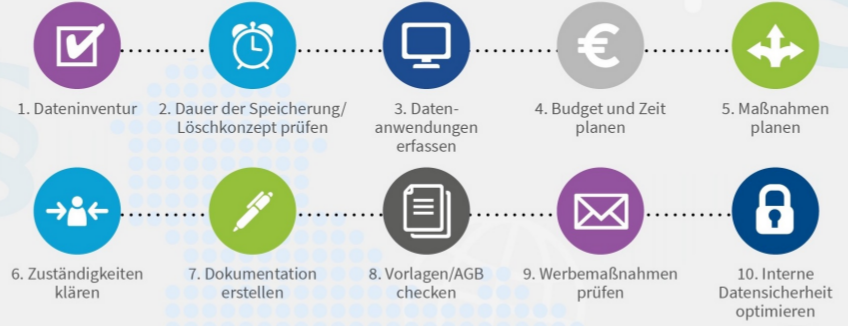
\includegraphics{figures/dsgvoSteps.png}
\caption{Steps DSGVO}
\end{figure}

\textbf{Grundlage jedes Datenschutz-Audits ist die Erhebung des
aktuellen Zustandes}:\\
Welche personenbezogenen Daten sind vorhanden? In welcher Form und wo?
Zu welchem Zweck? Wer zeichnet sich verantwortlich? Wer hat Zugang? Wie
lange werden diese gespeichert? Handelt es sich um besonders
schützenswerte Personendaten? Wie werden diese technisch \&
organisatorisch geschützt? Wie wird das Risiko einer Verletzung \& deren
Folgen beurteilt?

    \section{Internet am Arbeitsplatz}

\subsection{Hauptinteresse der Arbeitgeber}

Mitarbeiter sind \textbf{loyal} und nutzen ihre Arbeitszeit
\textbf{überwiegend} zum Vorteil des Arbeitgebers. Mitarbeiter halten
sensitive Informationen \textbf{vertraulich} und vermischen nicht
geschäftliche und private Daten.

\subsection{Hauptinteresse der Arbeitnehmer}

\begin{itemize}
\tightlist
\item Zugang zu den für die Arbeit notwendigen Informationen
\item Nicht von der ``privaten Welt'' abgeschnitten zu sein
\item Respekt der Privatsphäre der Arbeitnehmers durch den Arbeitgeber
\item Schutz der personenbezogenen Daten durch den Arbeitgeber
\end{itemize}

Art 328B im OR Regelt das Arbeitsverhältnis und der Datenschutz.

\subsection{Datenschutz \& Bewerbungsverfahren}

\textbf{Referenzauskünfte} sind nur mit \textbf{ausdrücklicher Zustimmung} des
Arbeitnehmers erlaubt.

\subsection{Überwachung des Arbeitnehmers (Art. 26 ArGV 3)}
\label{sec:IW-Überwachung}

\begin{enumerate}
	\tightlist
	\item Überwachungs- und Kontrollsysteme, die das \textbf{Verhalten} der
	Arbeitnehmer am Arbeitsplatz überwachen sollen, \textbf{dürfen nicht
	eingesetzt werden}.
	\item Sind Überwachungs- oder Kontrollsysteme aus anderen Gründen
	erforderlich, sind sie insbesondere so zu gestalten und anzuordnen,
	dass die \textbf{Gesundheit} und die \textbf{Bewegungsfreiheit} der
	Arbeitnehmer dadurch \textbf{nicht beeinträchtigt} werden.
\end{enumerate}

\subsection{Kontrolle der Kommunikation}

\textbf{Permanente} \& systematische \textbf{Kontrolle} der
Kommunikation (Internet, Email, Telefon) ist \textbf{illegal}. Wenn
\textbf{vorgängig angekündigt \& zeitlich eingeschränkt}, sind
Stichproben \& individuelle Kontrollen aber \textbf{zulässig}. Ausgenommen
davon sind strafrechtliche Untersuchungen von Behörden. Diese sind immer legal
sofern sie korrekt angeordnet wurden.

\mbox{}\\
Um allfälligen Problemen vorzubeugen ist es sinnvoll, den Arbeitnehmer einen
``Code of Conduct'' (Nutzungsreglement) unterzeichnen zu lassen.

\clearpage
\section{Whistleblowing}

\emph{Ein Whistleblower is a person who exposes any kind of information or
activity that is deemed illegal, unethical or not correct within an
organisation that is either private or public.} - Wikipedia

\mbox{}\\
Es mag illegal sein, solche Informationen aufzudecken, aber ethisch notwendig.
Das Aufdecken von solchen Informationen bedeutet grosse Risiken, sowohl für den
Whistleblower als auch für die betroffene Organisation.

\mbox{}\\
Wichtige Begriffe im Zusammenhang mit Whistleblowing sind:
\begin{description}
	\tightlist
	\item[Illegal] Verletzung einer Gesetzesbestimmung
	\item[Illegitim] Verletzung einer internen Regelung oder Direktive
	\item[Unethisch] Unmoralische \& unethische Praktiken
\end{description}

\subsection{Verpflichtung von Whistleblowing}
\label{sec:IW-Verpflichtungen}

\begin{itemize}
\tightlist
	\item Wenn ein Arbeitnehmer in seinem Verantwortungsbereich illegale
	Handlungen feststellt, so hat er seine Vorgesetzten zu informieren
	(\textbf{Treuepflichten}, Art. 321a Abs. 1 OR). Dieser Schritt lässt
	sich jedoch kaum jemandem Vorwerfen.
	\item \textbf{Beamte (des Bundes) sind verpflichtet}, ihre Vorgesetzten über
	alle festgestellten illegale Aktivitäten zu informieren (Art. 22a
	BPG).
	\item Wenn der WB mit seinen Feststellungen bei den Vorgesetzten keine
	Beachtung findet, so ist er zur Information der Öffentlichkeit nur
	berechtigt, wenn mehrere Voraussetzungen erfüllt sind!
	\textbf{(Proportionalität \& Kaskadenprinzip)}.
	\item \textbf{Corporate Governance \& Compliance/Risk Management verlangen
	ständige Sicherheitsüberprüfungen} (Art. 716a Abs. 1 OR). Eventuell sind die
	Regularien des Sarbanes-Oxley Acts (SOX) anwendbar.
	\item Es muss organisatorisch sichergestellt sein, dass der WB seine
	Anonymität behält, aber dennoch die Kommunikation mit ihm möglich ist!
\end{itemize}

\subsection{Rechtlicher Schutz des Whistleblowers}
\label{sec:IW-Schutz}
Zwar Schutz der Meinungsäusserungsfreiheit durch Art. 10 EMRK \& Art. 16
BV, aber in der Praxis Gefahr von strafrechtlicher Verfolgung. Aktuell wird
das OR überarbeitet um zusätzlichen rechtlichen Schutz für Whistleblower zu
schaffen. Die Gesetzesänderung ist aber noch nicht definitiv. Aktuell gibt
es nur geringen Schutz bei missbräuchlicher Kündigung durch eine ``Pönale'' von
Maximum 6 Monatslöhnen (Art. 336 OR).

\subsubsection{Entwurf Art. 321A OR}

Die Information der Öffentlichkeit über eine Unregelmässigkeit steht im Einklang
mit der Treuepflicht der Arbeitnehmerin oder des Arbeitnehmers, wenn:
\begin{itemize}
	\tightlist
	\item die Arbeitnehmerin oder der Arbeitnehmer ernsthafte Gründe hat, den
	gemeldeten Umstand in guten Treuen für wahr zu halten;
	\item sie oder er die Unregelmässigkeit vorgängig der zuständigen Behörde
	nach Artikel 321 oder 321 gemeldet hat; und
	\item eine der folgenden Voraussetzungen erfüllt ist:
	\begin{enumerate}
		\tightlist
		\item Die Arbeitnehmerin oder der Arbeitnehmer hat die zuständige
		Behörde ersucht, über die Behandlung der Meldung informiert zu werden
		und diese hat ihr oder ihm die geeigneten Auskünfte nicht innert
		vierzehn Tagen ab Erhalt des Ersuchens erteilt.
		\item Nach der Meldung an die Behörde wurde der Arbeitnehmerin oder dem
		Arbeitnehmer gekündigt oder sind ihr oder ihm andere Nachteile entstanden
	\end{enumerate}
\end{itemize}

    \section{Strafaspekte}

\subsection{Weshalb Strafrecht?}

\begin{itemize}
	\tightlist
	\item Gewaltmonopol als stabilisierende, kulturelle Leistung. Aber nur, wenn
	monopol demokratisch legitimiert ist und Verfahren und Sanktionen
	voraussehbar sind! Ziel des Strafrechts ist u.a. Abschreckung
	(„Generalprävention``) und individuelle Besserung
	(``Spezialprävention``).
	\item ``\textbf{nulla poena sine lege}'' (keine Strafe one Gesetz)
	\item Bestraft wird nur, wem (kumulativ!) \textbf{tatbestandmässiges},
	\textbf{rechtswidriges} und \textbf{schuldhaftes} Handeln nachgewiesen
	wurde.
\end{itemize}

\subsection{Für die Strafbarkeit sind immer zu prüfen}

\begin{enumerate}
	\tightlist
	\item Menschliche Handlung
	\item Tatbestandsmässig (objektiv/subjektiv)
	\begin{itemize}
		\tightlist
		\item Wurde objektiv betrachtet überhaupt etwas illegales gemacht?
		\item vorsätzlich/eventualvorsätzlich/fahrlässig (grob- oder
		leichtfahrlässig)
	\end{itemize}
	\item Rechtswidrig (Notwehr/Notstand)
	\begin{itemize}
		\tightlist
		\item \textbf{Notstand} bedeutet, wenn man in einer Not-Situation ist und
		sich durch eine strafbare Handlung in Sicherheit bringt. z.B. bei einem
		Sturm im Berg in eine Hütte einbrechen.
		\item \textbf{Notwehr} bedeutet, dass die Handlung stattfand als der Täter
		sein Leben/Gesundheit verteidigte
	\end{itemize}
	\item Schuldhaft (Schuldfähigkeit)
	\begin{itemize}
		\tightlist
		\item schuldunfähig/verminderte Schuldfähigkeit (Kinder sind
		beispielsweise beschränkt haftbar)
	\end{itemize}
	\item Mit Strafe/Sanktion bedroht
\end{enumerate}

\subsection{Sanktionen}
\subsubsection{Strafen}

\begin{itemize}
	\tightlist
	\item Freiheisstrafe (Vergehen <= 3 Jahre / Verbrechen >= 3 Jahre)
	\item Geldstrafe
	\item Gemeinnützige Arbeit
\end{itemize}

\subsubsection{Massnahmen}

Sind keine Strafen sondern Massnahmen zur Schutz der Gesellschaft.

\begin{itemize}
	\item therapeutische Massnahme (stationär/ambulant)
	\item Verwahrung
	\item Andere (Berufsverbot/Fahrverbot/Einziehung etc.)
\end{itemize}


\subsection{Strafzumessung}
\begin{itemize}
	\tightlist
	\item Freiheitsstrafen: 3 Tage bis 20 Jahre, z.T. lebenslänglich
	\item Geldstrafen: 1 Tagessatz bis 360 Tagessätze
	\item Gemeinnützige Arbeit: bis 720 Stunden
	\begin{itemize}
		\tightlist
		\item Vorallem im Jugendstrafrecht.
	\end{itemize}
	\item Busse: grundsätzlich bis 10'000.--- CHF, wenn gesetzlich vorgesehen
	aber auch höher
	\item Eine bedingte Haftstrafe kann mit einer unbedingten Geldstrafe/Busse
	verbunden werden!
\end{itemize}

Eine \textbf{bedingte} Haftstrafe kann mit einer unbedingten Geldstrafe/Busse
verbunden werden! Mehrere Taten (bspw. Einbruch = Hausfriedensbruch + Diebstahl)
wirken strafschärfend.

\subsubsection{Bedingt vs.~unbedingt}

Eine \textbf{unbedingte} Strafe wird vollzogen. Eine \textbf{bedingte}
Strafe wird nur vollzogen, wenn in einer Frist nochmals eine Tat
begannen wird. Die Handlung muss dabei nicht im selben Feld bestehen.

\subsection{Ablauf Strafverfahren}

\begin{itemize}
	\tightlist
	\item Polizei/Staatsanwaltschaft (StA) wird aktiv
	\item Untersuchungsleitun durch StA
	\item StA hat Aufgabe, belastende \& entlastende Aspekte zu untersuchen (im
	Zweifel klagt er jedoch an!)
	\item StA entscheidet, ob der Fall zur Beurteilung an Strafgericht
	überwiesen wird
	\item StA hat in einfachen Fällen Strafkompetenz
\end{itemize}

\subsection{Typische Cyber-Delikte}
\label{sec:CD-Overview}

\begin{itemize}
	\tightlist
	\item Unbefugte Datenbeschaffung (143 StGB)
	\item Unbefugtes Eindringen („Hacken``) in Datenverarbeitungssystem (143bis
	StGB)
	\item Datenbeschädigung (Art. 144bis StGB)
	\item Betrügerischer Missbrauch einer Datenverarbeitungsanlage (Art. 147
	StGB)
	\item Herstellen und Inverkehrbringen von Materialien zur unbefugten
	Entschlüsselung codierter Angebote (Art. 150Bis StGB)
	\item Verletzung des Fabrikations- oder Geschäftsgeheimnisses (Art. 162
	StGB)
	\item Ehrverletzungen (173ff StGB)
	\item Verletzung des Schriftgeheimnisses (179 StGB)
	\item Unbefugtes Beschaffen von Personendaten (179novies StGB)
	\item Pornografie (197 StGB)
	\item Störung von Betrieben, die der Allgemeinheit dienen (239 StGB)
	\item Rassendiskriminierung (261 bis StGB)
	\item Wirtschaftlicher Nachrichtendienst (273 StGB)
\end{itemize}

\subsubsection{Unbefugte Datenbeschaffung (Art. 143 StGB)}
\label{sec:CD-Datenbeschaffung}
\begin{enumerate}
	\tightlist
	\item Wer in der Absicht, sich oder einen andern unrechtmässig zu
	bereichern, sich oder einem andern elektronisch oder in
	vergleichbarer Weise gespeicherte oder übermittelte Daten
	beschafft, die nicht für ihn bestimmt und gegen seinen unbefugten
	Zugriff besonders gesichert sind, wird mit Freiheitsstrafe bis zu fünf
	Jahren oder Geldstrafe bestraft.
	\item Die unbefugte Datenbeschaffung zum Nachteil eines Angehörigen
	oder Familiengenossen wird nur auf Antrag verfolgt.
\end{enumerate}

\subsubsection{Unbefugtes Eindringen in ein Datenverarbeitungssystem (Art. 143bis StGB)}
\label{sec:CD-Eindringen}
\begin{enumerate}
	\tightlist
	\item Wer auf dem Wege von Datenübertragungseinrichtungen
	unbefugterweise in ein fremdes, gegen seinen Zugriff besonders gesichertes
	Datenverarbeitungssystem eindringt, wird, auf Antrag, mit Freiheitsstrafe
	bis zu drei Jahren oder Geldstrafe bestraft.
	\item Wer Passwörter, Programme oder andere Daten, von denen er weiss oder
	annehmen muss, dass sie zur Begehung einer strafbaren Handlung gemäss
	Absatz 1 verwendet werden sollen, in Verkehr bringt oder zugänglich
	macht, wird mit Freiheitsstrafe bis zu drei Jahren oder Geldstrafe bestraft.
\end{enumerate}

\subsubsection{Datenbeschädigung (Art. 144bis StGB)}
\label{sec:CD-Datenbeschädigung}
\begin{enumerate}
	\tightlist
	\item Wer unbefugt elektronisch oder in vergleichbarer Weise gespeicherte
	oder übermittelte Daten verändert, löscht oder unbrauchbar macht, wird,
	auf Antrag, mit	Freiheitsstrafe bis zu drei Jahren oder Geldstrafe bestraft.
	\\
	\\
	Hat der Täter einen grossen Schaden verursacht, so kann auf Freiheitsstrafe
	von einem Jahr bis zu fünf Jahren erkannt werden.
	Die Tat wird von Amtes wegen verfolgt.
	\item Wer Programme, von denen er weiss oder annehmen muss, dass sie zu den
	in Ziffer 1 genannten Zwecken verwendet werden sollen, herstellt, einführt,
	in Verkehr bringt, anpreist, anbietet oder sonst wie zugänglich macht oder
	zu ihrer Herstellung Anleitung gibt, wird mit Freiheitsstrafe bis zu drei
	Jahren oder Geldstrafe bestraft.\\
	\\
	Handelt der Täter gewerbsmässig, so kann auf Freiheitsstrafe von einem Jahr bis zu
	fünf Jahren erkannt werden.
\end{enumerate}

\subsubsection{Betrügerischer Missbrauch einer Datenverarbeitungsanlage
(Art. 147 StGB)}
\label{sec:CD-Missbrauch}
\begin{enumerate}
	\tightlist
	\item Wer in der Absicht, sich oder einen andern unrechtmässig zu bereichern,
	durch unrichtige, unvollständige oder unbefugte Verwendung von Daten oder
	in vergleichbarer Weise auf einen elektronischen oder vergleichbaren
	Datenverarbeitungs- oder Datenübermittlungsvorgang einwirkt und dadurch
	eine Vermögensverschiebung zum Schaden eines andern herbeiführt oder
	eine Vermögensverschiebung unmittelbar darnach verdeckt, wird mit
	Freiheitsstrafe bis zu fünf Jahren oder Geldstrafe bestraft.
	\item Handelt der Täter gewerbsmässig, so wird er mit Freiheitsstrafe bis
	zu zehn Jahren oder Geldstrafe nicht unter 90 Tagessätzen bestraft.
	\item Der betrügerische Missbrauch einer Datenverarbeitungsanlage zum
	Nachteil eines Angehörigen oder Familiengenossen wird nur auf Antrag verfolgt.
\end{enumerate}

\subsubsection{Herstellen \& Inverkehrbringen von Materialien zur unbefugten
Entschlüsselung codierter Angebote (Art. 150bis StGB)}
\label{sec:CD-Herstellen}
\begin{enumerate}
	\tightlist
	\item Wer Geräte, deren Bestandteile oder Datenverarbeitungsprogramme,
	die zur unbefugten Entschlüsselung codierter
	Rundfunkprogramme oder Fernmeldedienste bestimmt und
	geeignet sind, herstellt, einführt, ausführt, durchführt, in
	Verkehr bringt oder installiert, wird, auf Antrag, mit Busse
	bestraft.
	\item Versuch und Gehilfenschaft sind strafbar.
\end{enumerate}

\subsubsection{Ehrverletzungs Delikte (Art. 173/174/177 StGB)}
\label{sec:CD-Ehrverletzung}
\begin{description}
	\tightlist
	\item[Üble Nachrede (Art. 173 StGB):] Der Straftatbestand hat zum Ziel,
	jemanden zu bestrafen, der gegenüber Dritten über eine andere Person
	\textbf{rufschädigende vorsätzlich wahre} (oder unvorsätzlich, d.h. gutgläubig
	unwahre) \textbf{Äusserungen tätigt oder weiterverbreite}t. Der Täter kann sich
	allerdings entlasten und bleibt straflos, wenn ihm der sogenannte
	\textbf{Entlastungsbeweis} (wahr \& öffentliches Interesse) gelingt.
	\item[Verleumdung (Art. 174 StGB)] Die Verleumdung ist üble Nachrede
	\textbf{wider besseren Wissens}. Der Täter beschuldigt oder verdächtigt eine
	Person gegenüber Dritten eines unehrenhaften Verhaltens oder anderer
	rufschädigender Tatsachen, die in Wirklichkeit nicht bestehen und somit
	unwahr sind. Der Entlastungsbeweis ist nicht möglich.
	\item[Beschimpfung (Art. 177 StGB)] Der Beschimpfung macht sich strafbar,
	wenn jemand in anderer Weise – d.h. nicht durch üble Nachrede oder
	Verleumdung – \textbf{durch Wort, Schrift, Bild, Gebärde oder Tätlichkeiten
	in der Ehre angegriffen} wird.
\end{description}

\subsection{Tipps}

\begin{itemize}
	\tightlist
	\item Bei Antragsdelikten nicht warten – \textbf{Frist von 90 Tagen!}
	\item Strafanzeige vs. zivilrechtliche Klagen gut abwägen
	(Zeit/Kosten/Nebenfolgen)
	\item Nur \textbf{Privatkläger} erhält Informationen aus der Untersuchung!
	\item Was einmal „unglücklich“ formuliert in den Befragungsprotokollen ist,
	lässt sich kaum korrigieren!
	\item i.d.R. ist Kooperation besser, als Aussageverweigerung! Aber als
	Beschuldigte/r muss man sich nicht belasten!
	\item Notfallplan „Hausdurchsuchung“ vorbereiten!
\end{itemize}


    \section{Grundzüge der industrierelevanten Verträge}

\subsection{Vertragstypen Übersicht}

\begin{tabular}{l|l|l|l}
Veräusserung & Gebrauchsüberlassung & Arbeitsleistung &
Übrige\\\hline
Kaufvertrag & AirBnB & Werkvertrag & Lizenzverträge \\
& Darlehen & Arbeitsvertrag & \\
& Mietvertrag & Auftrag & \\
\end{tabular}

\subsection{Verträge auf Arbeitsleistung}

\subsubsection{Arbeitsvertrag (Art. 319-362 OR)}

\begin{description}
	\item[Grundsätze] \mbox{}
	\begin{itemize}
		\tightlist
		\item Verrichtung von Arbeit nach Weisungen des Arbeitgebers
		\item Risiko liegt beim Arbeitgeber
	\end{itemize}
	\item[Lohn] Lohnanspruch
	\item[Auflösung] Kündigungsfrist
\end{description}

\subsubsection{Werkvertrag (Art. 363-379 OR)}

\begin{description}
	\item[Grundsätze] \mbox{}
	\begin{itemize}
		\tightlist
		\item Die Pflicht für einen Auftraggeber ein Werk zu erstellen (bspw.
		Software)
		\item Das Entscheidende bei einem Werkvetrag ist das Resultat
		-> Erfolgsverschulden
	\end{itemize}
	\item[Lohn] Vergütungsanspruch
	\item[Auflösung] Jederzeit, solange Werk nicht vollendet
\end{description}

\subsubsection{Auftrag (Art. 394-418v OR)}

\begin{description}
	\item[Grundsätze] \mbox{}
	\begin{itemize}
		\tightlist
		\item Besorgung von Geschäften im Interesse des Auftraggebers
		\item Weisungsrecht des Auftraggebers
		\item Sorgfältige Ausführung, aber kein Erfolg geschuldet
	\end{itemize}
	\item[Lohn] Falls verabredet oder üblich
	\item[Auflösung] Jederzeit, zwingendes Kündigungsrecht
\end{description}

\subsection{Werkvertrag}

\subsubsection{Mängelrechte}
\label{sec:Werkvertrag-Mängelrechte}
\begin{figure}[H]
	\centering
	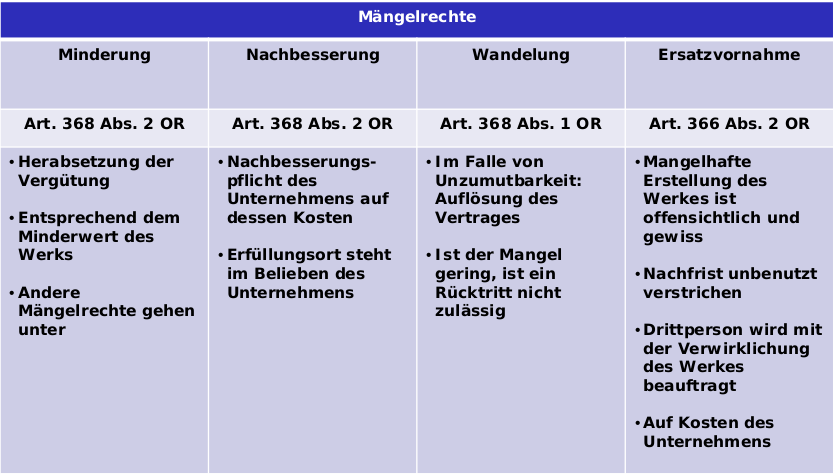
\includegraphics[width=.9\textwidth]{figures/maengelRechte.png}
	\caption{Mängelrechte Werkvertrag}
\end{figure}

\paragraph{Ersatzvornahme}\mbox{}\\
Wird ein Meilenstein während dem laufenden Werkvertrag nicht erreicht,
muss zuerst eine angemessene Nachfrist vereinbart werden. Wird diese
Nachfrist nach wie vor nicht genutzt und verstrichen, kann ein
Dritt-Unternehmen zur Lösung des Problems angestellt werden und die
Kosten müssen durch den Werkvertrag-Nehmer übernommen werden.

\mbox{}\\
Drei Dinge, die bei einem Werkvertrag als erstes beachtet werden
sollten:
\begin{enumerate}
	\tightlist
	\item Zwischen wem ist der Vertrag?
	\item Welches Recht und welcher Gerichtsstand gilt?
	\item Wie komme ich wieder aus dem Vertrag raus?
\end{enumerate}

\subsubsection{Preisvereinbarung}
\label{sec:Werkvertrag-Preisvereinbarung}

\paragraph{Vereinbarter Preis (Art. 373 OR)}
\begin{description}
	\item[Pauschalpreis] Vertraglich fixierter Betrag als Höchst- und
	Mindestpreis.
	\item[Globalpreis] Festpreis (Teuerung angepasst)
	\item[Ausnahme] Missverhältnis zwischen Leistung und Vergütung\\
	Keine Voraussehbarkeit der Umstände.
\end{description}

\paragraph{Fehlende Preisvereinbarung (Art. 374 OR)}

\begin{itemize}
	\tightlist
	\item Wert der Arbeit und der Aufwendungen sind die Vergütungsbemessung
	massgebend (z.B. unverbindlicher Kostenvoranschlag). Ein solcher
	Kostenvoranschlag hat eine gewisse Bedeutung, damit das Kostenrisiko nicht
	ganz auf den Besteller übergeht.
	\item Achtung: Art. 375 Abs. 1 OR: Rücktrittsrecht des Bestellers, wenn
	\textbf{wesentlich} überschritten. (wesentlich = 10\%)
\end{itemize}

\subsubsection{Pflichten des Unternehmners resp. Bestellers}
\label{sec:Werkvertrag-RechtePflichten}

\paragraph{Pflichten des Unternehmers}

\begin{itemize}
	\tightlist
	\item  Pflicht zur Herstellung eines Werks (Art. 363 OR)
	\begin{itemize}
		\tightlist
		\item  Materielles Werk: bewegliche oder unbewegliche Sache
		\item Geistiges Werk: wissenschaftliche oder künstlerische Leistungen
	\end{itemize}
	\item Pflicht zur Lieferung des Werks (Art. 367 OR)
	\begin{itemize}
		\tightlist
		\item Erfolg geschuldet:
		Resultat muss nach obj. Kriterien überprüft und als richtig oder falsch
		qualifiziert werden können
	\end{itemize}
	\item keine besonderen Treuepflichten
\end{itemize}

\paragraph{Pflichten des Bestellers}
\begin{itemize}
	\tightlist
	\item  Pflicht zur Annahme und Abnahme des Werks (Art. 370 OR)
	\begin{itemize}
		\tightlist
		\item  Werkmangel: Vertragliche zugesicherte Eigenschaften fehlen
		\begin{itemize}
			\tightlist
			\item Wertqualität: normale Beschaffenheit
			\item Gebrauchsqualität: normale Benutzung
		\end{itemize}
		\item Prüfungspflicht innert nützlicher	Frist, ansonsten
		Genehmigungsfiktion!
	\end{itemize}
	\item Pflicht zur Leistung einer Vergütung (Art. 363 u. 372 OR)
\end{itemize}

\subsection{Auftrag}
\label{sec:Auftrag-Overview}
Ein Auftrag erfordert eine \textbf{sorgfältige Ausführung}. Es wird jedoch
\textbf{kein Erfolg geschuldet}.

Der Auftrag muss persönlich ausgeführt werden. Andernfalls musst der
Beauftragte den Auftraggeber informieren, falls die ausführende Person
wechselt.

\begin{figure}[H]
	\centering
	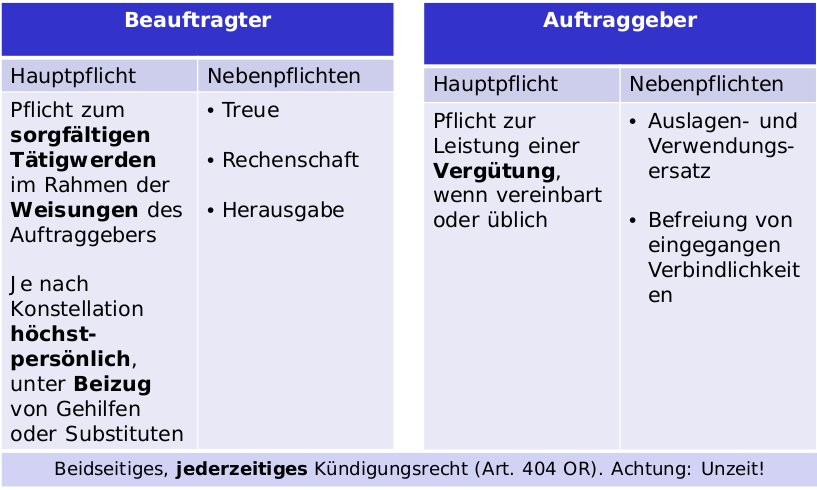
\includegraphics[width=.9\textwidth]{figures/auftraggeberBeauftragter.png}
	\caption{Beauftragter und Auftraggeber}
\end{figure}

\begin{description}
	\item[Herausgabe] Der Arzt z.B. die Dossiers an
	einen neuen Arzt weitergibt oder Informationen zur Verfügung stellt.
	\item[Unzeit] Die Gegenseite kann nicht mehr disponieren.
	\item[Kündigung] Jederzeit, \textbf{unabhängig davon ob Kündigungsfristen
	im Auftrag stehen} oder nicht.
\end{description}


\subsection{Vertragsabschluss}

\subsubsection{Voraussetzungen}

\begin{enumerate}
	\tightlist
	\item \textbf{Rechts- und Handlungsfähigkeit} der Vertragsparteien
	\item Vorliegen \textbf{beidseitigen Geschäftswillen}
	\item \textbf{Austausch übereinstimmender Willenserklärungen}
	\begin{itemize}
		\tightlist
		\item Antrag:
		\begin{itemize}
			\tightlist
			\item Zeitlich erste Willenserklärung bei Vertragsverhandlung
			\item Muss alle für den Vertrag massgebenden Punkte enthalten
		\end{itemize}
		\item Annahme:
		\begin{itemize}
			\tightlist
			\item Zeitlich zweite Willenserklärung bei der Vertragsverhandlung
			\item Antragsempfänger erklärt Willen zum Vertragsabschluss durch die
			Annahme
			\item Inhaltliche Übereinstimmung von Antrag und Annahme notwendig
		\end{itemize}
	\end{itemize}
	\item Einhaltung von Formvorschriften, sofern erforderlich\\
	Gewisse Verträge müssen z.b. schriftlich, öffentlich oder beurkundet
	werden.
	\item Keine Verletzung inhaltlicher Schranken / keine Willensmängel (Art.
	19/20ff. OR)
\end{enumerate}


\subsubsection{Formvorschriften}

\begin{figure}[H]
\centering
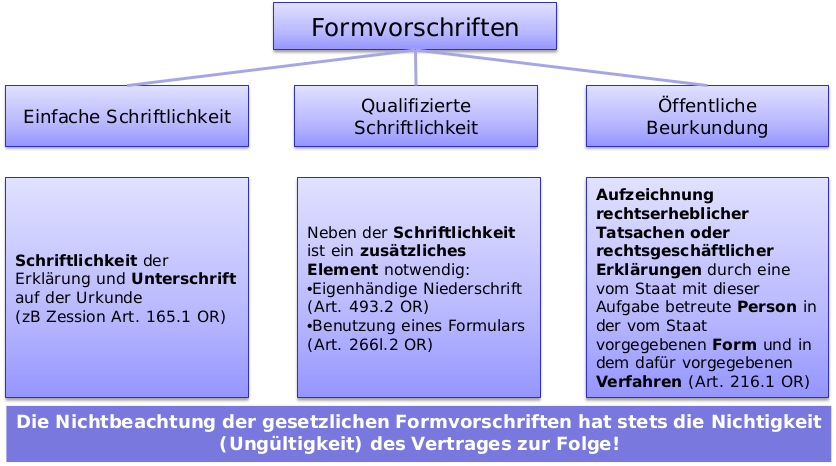
\includegraphics[width=.9\textwidth]{figures/formvorschriftenVertragsabschluss.png}
\caption{Formvorschriften Vertragsabschluss}
\end{figure}

Ein Mail entspricht nicht \textbf{einfacher Schriftlichkeit}.\\
Ein Testament muss z.B. handschriftlich (Qualifizierte Schriftlichkeit)
sein, sonst ist es formnichtig.\\
Eine Kündigung eines Mietverhältnisses durch den Vermieter muss mit
einem offiziellen Formular gemacht werden (Qualifizierte
Schriftlichkeit).

\subsubsection{Vertragserfüllung}

\begin{itemize}
\tightlist
\item Bei der Vertragserfüllung werden die durch den Vertragsabschluss
begründeten Obligationen (Verpflichtungen) erfüllt.
\item Das Internet ist ein neues Kommunikationsmedium, das heute vermehrt
dazu benutzt, übereinstimmende Willensäusserungen auszutauschen, die
zu Vertragsabschlüssen führen (Art. 1 OR).
\item Fragen des Vertragsabschlusses und der Vertragserfüllung regeln sich
-- genau wie beim mündlichen Vertragsabschluss oder beim brieflichen
Austausch von Willenserklärungen -- nach den allgemeinen Bestimmungen
des Obligationenrechts.
\end{itemize}

\subsubsection{Vertragsverletzungen}

\begin{figure}[H]
\centering
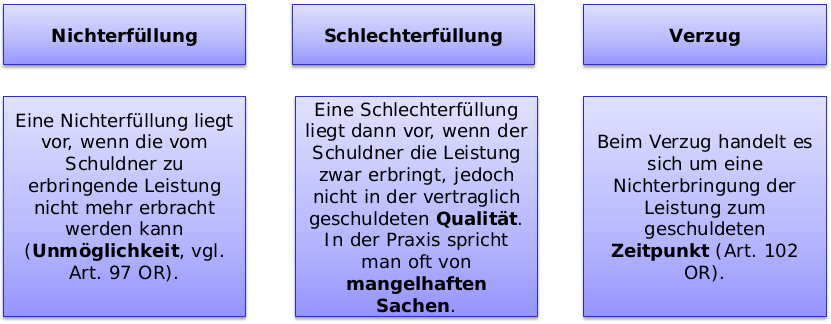
\includegraphics[width=.8\textwidth]{figures/agbVertragsverletzungen.png}
\caption{AGB Vertragsverletzung}
\end{figure}

\textbf{Knonentionalstrafe:} Ist unabhängig ob wirklich ein Schaden
entstanden ist oder nicht. Zudem kann zusätzlich die Vertragserfüllung
trotzdem verlangt werden.

\subsection{AGB}

AGB sind \textbf{vorformulierte} Vertragsbestimmungen, die als Grundlage
für eine Vielzahl von Verträgen verwendet werden, die der Verfasser mit
seinen Kunden schliesst.

Ziele von AGB:
\begin{itemize}
	\tightlist
	\item \textbf{Rationalisierungszweck}
	\item Besserstellungszweck:
	\begin{itemize}
		\tightlist
		\item Freizeichnungs-Klauseln
		\item  Sicherheiten-Klauseln
		\item Risikoverlagerungen
	\end{itemize}
	\item Verhandlungsvorgabe
\end{itemize}


\subsubsection{Einbezug}
Für das Zustandekommen eines Vertrages (Konsens) bedarf es der
übereinstimmenden gegenseitigen Willenserklärungen beider Parteien. Dies
gilt auch für die Einbeziehung der AGB in den Individualvertrag

\paragraph{Voraussetzungen der AGB-Einbeziehung}
\begin{itemize}
	\item AGB-Kundbarmachung:
	Kunde \textbf{ist vor oder während} der Vertragsverhandlungen auf die
	AGB hinzuweisen
	\item AGB-\textbf{Kenntnisnahme}: Kunde muss spätestens vor
	Vertragsschluss Gelegenheit zur Kenntnisnahme haben.\\
	Achtung: Nachgeschobene AGB sind ungültig
	\item AGB-Geltung: Kunde muss mit der AGB-Geltung einverstanden sein.
\end{itemize}


\subsubsection{Typologisierung}
\begin{figure}[H]
\centering
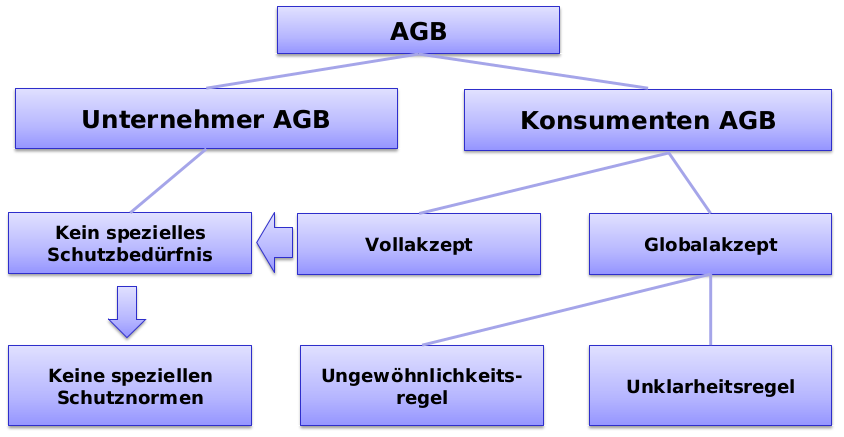
\includegraphics[width=.9\textwidth]{figures/typolisierungAGB.png}
\caption{Typologisierung der AGB}
\end{figure}

\begin{description}
	\item[Globalakzept] Bedeutet, dass viele leute einfach ohne zu lesen
	die AGB akzeptieren. Dann gibt es die beiden folgenden Regeln zu
	beachten.
	\item[Ungewöhnlichkeits- und Unklarheitsregel]
	Verwendung missbräuchlicher Geschäftsbedingungen (Art. 8 UWG) „Unlauter
	handelt insbesondere, wer allgemeine Geschäftsbedingungen verwendet, die
	in \textbf{Treu und Glauben} verletzender Weise zum Nachteil der
	Konsumentinnen und \textbf{Konsumenten} ein erhebliches und
	ungerechtfertigtes \textbf{Missverhältnis} zwischen den vertraglichen
	\textbf{Rechten und Pflichten} vorsehen.``
	\item[Ungewöhnlichkeitsregel]  Enthalten AGB Bestimmungen, mit denen
	der Kunde (nach Treu und Glauben) nicht rechnen muss, so sind diese
	Bestimmungen für den Kunden nicht verbindlich\\
	\emph{z.B. in einem Ski-Hüttchen der Gerichtsstand in Florida}
	\item[Unklarheitsregel] Finden sich in den AGB Regelungen, die unklar
	sind, so werden diese zu Lasten des Verfassers der AGB ausgelegt.\\
	\emph{Wenn der Leser etwas der AGBs nicht versteht (oder verstehen
	kann), werden diese Teile zu Lasten des Verfassers ausgelegt.}
\end{description}


\subsection{SIA-Verträge}

\begin{itemize}
	\tightlist
	\item Vertragsformulare der SIA für Geschäftsbeziehungen zwischen
	\begin{itemize}
		\tightlist
		\item \textbf{Bauherren und Planern} (Aufträge) sowie zwischen
		\begin{itemize}
			\tightlist
			\item BSP: Vertrag für Ingenieurleistungen Nr. 1003
		\end{itemize}
		\item \textbf{Bauherren und Unternehmern} (Werkverträge)
		\begin{itemize}
			\tightlist
			\item BSP: Werkvertrag Nr. 1023
		\end{itemize}
	\end{itemize}
	\item Sicherstellung der \textbf{korrekten Einbindung} der entsprechenden
	Vertragsnorm
	\item \textbf{Breit abgestützte Grundlage} für die Geschäftsbeziehung
	\item Schweizweit anerkannt und für \textbf{80\% der Fälle als Standard
	anwendbar}
	\item Knappe und \textbf{klare Struktur} / detaillierte Aspekte mithilfe von
	Beilagen
\end{itemize}

\subsection{SWICO-Verträge}

\begin{itemize}
	\tightlist
	\item IT-Modellverträge, welche durch Anwälte der Verbände SWICO und
	SwissICT erarbeitet werden
	\item Faire und ausgewogene Regelungen
	\item Konkrete Bezugnahme auf IT-relevante Vertragsgestaltungen
	\item Nur Geltung, wenn konkret im Vertrag vereinbart
\end{itemize}

\textbf{Vorteile Swico-Verträge}

\begin{enumerate}
	\tightlist
	\item Branchenbezogenheit
	\item Fachgerechte Formulierung
\end{enumerate}

    \section{Grundzüge des Markenrechts}

Die Marke ist ein Zeichen, das geeignet ist, Waren oder Dienstleistungen
eines Unternehmens von solchen anderer Unternehmen zu unterscheiden.

Marken können insbesondere Wörter (Siemens), Buchstaben (SBB), Zahlen
(501 -> Lewis), bildliche Darstellungen (Swisscom),
dreidimensionale Formen oder Verbindungen solcher Elemente untereinander
oder mit Farben sein.

\subsection{Form}

\begin{itemize}
\tightlist
\item Wortmarke
\item Bildmarke
\item Kombinierte Wort-/Bildmarke
\item Formmarke
\end{itemize}

\subsection{Unterscheidung nach Zweck}

\begin{description}
	\tightlist
	\item[Individualmarke] Marke eines einzelnen Unternehmens für eine
	bestimmte Ware oder Dienstleistung
	\item[Garantiemarke]  Gewährleistung gewisser Produkteigenschaften
	zB: ZEWO
	\item[Kollektivmarke] Kennzeichnung der Produkte einer Vereinigung
	zB: Fleurop, FMH
\end{description}

\subsection{Schutzvoraussetzungen}

\subsubsection{Absolute Ausschlussgründe}

Wenn eine der folgenden Bedingungen eintritt, kann eine Marke
\textbf{nicht registriert} werden:

\begin{enumerate}
	\tightlist
	\item Zeichen des Gemeingutes
	\begin{itemize}
		\tightlist
		\item Sachbezeichnungen: Marken, die ein Produkt bloss beschreiben oder
		eine Sache als diese Sache benennen.\\
		(z.B. Apple für Äpfel)
		\item Freizeichen: Zu Schabezeichnungen ``degeneriert'' oder Konkurrenten
		sind auf die Verwendung dieser Zeichen angewiesen\\
		(z.B. Fön, Linoleum oder Nylon)
	\end{itemize}
	\item Allgemein notwendige Formen: Formen, die das Wesen der Ware ausmachen
	oder technisch notwendig sind (z.B. Fussball)
	\item Irreführende Zeichen: Falsche Erwartungen betreffend Herkunft,
	Qualität oder geschäftlicher Verhältnisse (z.B. Kübler-Rad)
	\item Zeichen gegen die öffentliche Ordnung/guten Sitten
	\item Wappen und andere öffentliche Zeichen
\end{enumerate}

\subsubsection{Relative Ausschlussgründe}

Die Marke wird auf Antrag eines Dritten (Widerspruch) nicht registriert,
wenn identische oder ähnliche Kennzeichen mit gleichen oder
gleichartigen Produkten vorliegen.

--> Verwechslungsgefahr

\mbox{}\\
Wenn eine Person eine Marke beantragt, ist er selber dafür
verantwortlich, dass seine Markenrechte nicht verletzt werden. Man muss
innerhalb von 3 Monaten klagen.


\subsubsection{Verwechslungsgefahr}

\begin{itemize}
	\tightlist
	\item Arten der Verwechslung
	\begin{description}
		\tightlist
		\item[Optik] Wortlänge und Art der Buchstaben
		\item[Akustik] Silbenmass, Aussprachekadenz, Vokalfolge\\
		zB: ''Tobler-o-rum'' / ''Torero-Rum''
		\item[Sinngehalt] Vermittlung von ''Ersatz für'' oder ''gleich gut wie''
	\end{description}
	\item Kennzeichenstärke: Starke Marken haben grösseren Schutzumfang
	\item Adressaten: Sicht des Kaufentscheidfällers
	\item Erinnerungsvermögen der Adressaten: bei Massenartikeln ist
	Verwechslungsgefahr grösser als bei Spezialprodukten / Aufmerksamkeit im
	Schmuckgeschäft höher als im Warenhaus
	\item Massgebend ist der Gesamteindruck beim durchschnittlichen Abnehmer
\end{itemize}

\emph{Die Hinterlegung einer gleichen Marke für völlig verschiedene
Produkte ist grundsätzlich möglich. Je ähnlicher sich die Produkte sind,
desto stärker müssen sich die Marken voneinander unterscheiden.}

\subsection{Registrierung}
\label{sec:Markenrecht-Registrierung}

Markenschutz ist \textbf{territorial}: Schutz nur in dem Land, in dem
Marke registriert ist. In der Schweiz regelt diese das Eisg. Institut für
Geistiges Eigentum (ige). Die meisten Länder werden jedoch von der
IGE -> World Intellectual Property Organziation verwaltet.

\begin{description}
	\item[Eintragungsprinzip] Die Marke entsteht erst mit der Eintragung
	ins Register (Art. 5 MSchG). Eine Ausnahme bildet die \textbf{notorisch
	bekannte Marke}\\
	Bsp: «Galeries Lafayette» vs. «Lafayette Chocolatier en
	Suisse». Marke war in der Schweiz eigentlich nicht geschützt, bekam jedoch in
	einem Streit recht, da sie weit verbreitet war.
	\item[Spezialitätenprinzip] Marke muss einer oder mehreren Waren oder
	Dienstleistungen zugewiesen werden und ist in der Folge lediglich für
	diese Verwendung geschützt (www.ige.ch). Eine Ausnahme bildet die
	berühmte Marke (Art. 15 MSchG).
	\item[Berühmte Marken] Die Marke ist zwar nur für eine Kategorie
	eingetragen, ist aber so bekannt, dass sie für sämtliche
	Markenkategorien geschützt ist. Bsp: Coca Cola.
\end{description}

Markenrechte erhält man für 10 Jahren und können jeweils um weitere 10
Jahre verlängert werden. Ein Markenrecht kann so unendlich lange
verlängert werden (sofern die Gebühren bezahlt werden).

    \section{Designrecht}

\subsection{Rechtsgrundlage}
\label{sec:Designrecht-Grundlage}

\paragraph{Art. 1 DesG}
Gestaltungen von Erzeugnissen oder Teilen von Erzeugnissen, die namentlich durch die Anordnung von Linien, Flächen, Konturen oder Farben oder durch das verwendete Material charakterisiert sind.\\

Designs stellen die bestimmte äussere Formgebung von etwas -
Zweidimensionalem (Muster) oder von etwas\\
zB: Gestaltung eines Stoffmusters, eines Uhrenzifferblatts oder einer
Flaschenetikette - Dreidimensionalem (Modell) dar\\
zB: die Form einer Zahnbürste, einer Lampe oder eines Stuhls


\subsection{Schutzvoraussetzungen}

\begin{enumerate}
	\tightlist
	\item Neuheit
	\begin{itemize}
		\tightlist
		\item In der Schweiz bisher nicht bekannt
		\item Keinem offenen, zahlenmässig unbeschränkten Personenkreis
		präsentiert (innerhalb 12 Monate nach Markteintritt muss das Deisgn
		registiert werden)
	\end{itemize}
	\item Eigenart
	\begin{itemize}
		\tightlist
		\item Unterscheidung von bisherigen ähnlichen Gestaltungen
		\item Geringere Anforderung an Originalität, als beim URG
	\end{itemize}
	\item Nicht gesetzeswidrig oder anstössiger Natur
\end{enumerate}

\subsubsection{Ausschlussgründe}

Die Merkmale des Designs dürfen nicht ausschliesslich durch die
technische Funktion des Erzeugnisses bedingt sein.\\
--> Formgebung darf nicht durch die technische Funktion
gegeben sein.

\subsection{Registrierung}
\label{sec:Designrecht-Registrierung}

\begin{description}
	\tightlist
	\item[Schweiz] Eidgenössisches Institut für Geistiges Eigentum 
	(ige). Kosten: 200 CHF
	\item[International] World Intellectual Property Organization
	(wipo)
\end{description}

Das Designrecht entsteht mit der Eintragung im Design-Register
(Art. 5 DesG).


\subsubsection{Hinterlegungspriorität}
\label{sec:Designrecht-Hinterlegungsprioritaet}

Das Designrecht steht demjenigen zu, der das Design zuerst hinterlegt
(Art. 6 DesG).

Zur Hinterlegung berechtigt ist diejenige Person, die das Design
entworfen hat, deren Rechtsnachfolgerin oder eine Drittperson, welcher
das Recht aus einem andern Rechtsgrund gehört.\\
Gemeinschaftliche Hinterlegung bei gemeinsamen Design möglich.

\subsection{Schutzdauer}

5 Jahre vom Datum der Hinterlegung an. Möglichkeit der Verlängerung um
4 Schutzperioden von je 5 Jahren. Maximaler Designschutz: 25 Jahre

\subsection{Rechtsschutz}

\begin{itemize}
	\tightlist
	\item Beschwerde an das Bundesverwaltungsgericht
	\begin{itemize}
		\tightlist
		\item gegen Verfügungen des IGE
	\end{itemize}
	\item Zivilverfahren (vgl. Markenrecht)
	\item Strafverfahren
	\item Hilfeleistung der Zollverwaltung
\end{itemize}

\section{Patentrecht}
\label{sec:Patentrecht-Zweck}

Das Patentrecht schützt Erfindungen und gewährt dem Inhaber das
ausschliessliche Recht, die durch das Patent geschützte Erfindung
gewerbsmässig zu nutzen (Art. 1 Abs. 1 PatG).\\
Das bedeutet auch, dass der Patentinhaber allen anderen die Nutzung
derselben Erfindung verbieten darf (Art. 8 PatG).

Der Schutz von Erfindungen soll in zweierlei Hinsicht den technischen
Fortschritt fördern:
\begin{itemize}
	\tightlist
	\item Zum einen bietet das Patent \textbf{Grundlage und Anreiz
	für Investitionen} in Forschung und Entwicklung, da Erfindungen mit dem
	Patent \textbf{geschützt} und \textbf{belohnt} werden.
	\item Zum andern ist die Beschreibung
	der Erfindung in der \textbf{Patentschrift öffentlich zugänglich}, was
	wiederum \textbf{innovationsfördernd} wirken soll.
\end{itemize}


\subsection{Patentarten}

\begin{description}
	\tightlist
	\item[Erzeugnispatent]  Bestimmter Gegenstand mit bestimmten Eigenschaften\\
	(z.B. eine chemische Substanz oder eine Maschine)
	\item[Verfahrenspatent] Zeitliches Aufeinanderfolgen von Geschehnissen\\
	(z.B. Verfahren zur Herstellung eines chemischen Stoffes oder zur
	Bearbeitung eines Metalls)
\end{description}


\subsection{Rechtsgrundlage}
\label{sec:Patentrecht-Rechtsgrundlage}

\begin{itemize}
\tightlist
\item Für neue gewerblich anwendbare Erfindungen werden Erfindungspatente
erteilt.
\item Was sich in nahe liegender Weise aus dem Stand der Technik (Art. 7
Abs. 2) ergibt, ist keine patentierbare Erfindung.
\item Die Patente werden ohne Gewährleistung des Staates erteilt.
\end{itemize}


\subsection{Schutzvoraussetzungen}

\begin{enumerate}
	\tightlist
	\item  Gewerbliche Anwendbarkeit: Alle Erfindungen, die zur Ausübung einer
	Erwerbstätigkeit angewendet werden können
	\item Neuheit: Nicht Stand der Technik (weltweit!)
	\begin{itemize}
		\tightlist
		\item Ausnahme: Unschädliche Offenbarung (Art. 7b PatG) mit Frist 6 Monate
		\item Offensichtlicher Missbrauch, bspw. Verstoss gegen Geheimhaltung
		\item Zurschaustellung an einer offiziell anerkannten Ausstellung
	\end{itemize}
	\item Erfindung: Lehre, wie sich eine Aufgabe durch den Einsatz von
	Naturstoffen und/oder Naturkräften wiederholbar lösen lässt.
	\begin{itemize}
		\tightlist
		\item ''Lösung für ein technisches Problem oder technische Lösung für ein
		Problem''
		\item Für Fachmann nicht naheliegend\\
		Als naheliegend gilt eine Erfindung, wenn eine durchschnittliche
		Fachperson, die mit derselben Problemstellung konfrontiert würde,
		ausgehend vom nächstliegenden Stand der Technik, dieselbe Lösung
		mittels der im betreffenden Gebiet bekannten oder logischen
		Vorgehen, d.h. ohne eigene erfinderische Leistung, aus dem Stand der
		Technik am Anmelde- oder Prioritätsdatum herleiten könnte bzw.
		würde.
	\end{itemize}
\end{enumerate}


\subsection{Was ist nicht patentierbar?}

\begin{itemize}
	\tightlist
	\item Nicht patentierbar sind Ideen, Konzepte, Entdeckungen,
	wissenschaftliche Theorien und mathematische Methoden.
	\item Computerprogramme «als solche » sind ebenfalls nicht patentierbar,
	hingegen können computerimplementierte Erfindungen unter Umständen
	patentierbar sein wie z.B. wie das Betriebssystem Windows.
	\item Anmeldung eines Computerprogramms beim Europäischen Patentamt (Art. 52
	Abs. 2 EPÜ) in Ausnahmefällen möglich, z.B. wenn das Computerprogramm
	«(mehrfachen) technischen Charakter» aufweist.
	\item Ebenfalls von der Patentierung ausgeschlossen sind Erfindungen, deren
	Verwertung gegen die öffentliche Ordnung oder die guten Sitten
	verstösst, wie dies z.B. beim Klonen von Menschen der Fall ist.
\end{itemize}


\subsection{Gesetzliche Begrenzung}
\label{sec:Patentrecht-Begrenzug}

Das Patentgesetz listet eine Reihe von Nutzungsarten auf, welche auch
mit Bezug auf patentierte Erfindungen, explizit zulässig sind (Art. 9
PatG):
\begin{itemize}
	\tightlist
	\item Handlungen im privaten Bereich zu nicht gewerblichen Zwecken
	\item Handlungen zu Forschungs- und Versuchszwecken, die der Gewinnung von
	Erkenntnissen über den Gegenstand der Erfindung, einschliesslich seiner
	Verwendungen, dienen (Forschungsprivileg)
	\item Benützung der Erfindung zu
	Unterrichtszwecken an Lehrstätten
\end{itemize}

\subsection{Freie Erfindung}
Eine Erfindung, welche in der Freizeit gemacht wurde. Eigentümer ist der Erfinder.

\subsection{Arbeitnehmererfindungen}
\label{sec:Patentrecht-Arbeitnehmererfindungen}
\begin{description}
	\item[Diensterfindungen] Sind Erfindungen des Arbeitnehmers, die er
	bei Ausübung einer dienstlichen Tätigkeit und in Erfüllung einer
	vertraglichen Pflichten macht oder an deren Hervorbringung er mitwirkt
	(Art. 332 Abs. 1 OR).
	\begin{itemize}
		\item Eigentum bei Arbeitgeber.
		\item Es besteht kein Anspruch auf finanzielle Entschädigung
		durch den Arbeitgeber.
	\end{itemize}
	\item[Gelegenheitserfindungen] Sind Erfindungen, die der Arbeitnehmer
	in Ausübung der dienstlichen Tätigkeit macht, dies jedoch ausserhalb
	seiner vertraglichen Pflichten.
	\begin{itemize}
		\tightlist
		\item Ohne Vereinbarung: Rechte beim Erfinder (Arbeitnehmer) (Art. 332 Abs.2
		OR).
		\item Mit vorheriger (!) Vereinbarung: Erwerb durch Arbeitgeber für
		angemessene Entschädigung möglich (Art. 332 Abs. 2 OR). Frist 6
		Monate.
		\item Umstände zur Bestimmung der angemessenen Entschädigung
		\item der wirtschaftliche Wert der Arbeitnehmererfindung
		\item die Mitwirkung des Arbeitgebers
		\item die Inanspruchnahme von betrieblichen Hilfspersonen und die
		Aufwendungen des Arbeitnehmers
		\item seine Stellung im Betrieb (Art. 332 Abs. 4 OR).
	\end{itemize}
\end{description}

\subsection{Schutzdauer und Rechtsschutz}
Ein Patent gilt \textbf{20 Jahre ab Anmeldedatum} und ist grundsätzlich
nicht erneuerbar. Ausnahme ist das \textbf{ergänzende Schutzzertifikat}
von zusätzlichen \textbf{fünf Jahren für Arznei- und Pflanzenschutzmittel}
aufgrund des langsamen Bewilligungsverfahren.\\

Rechtlicher Schutz:\\
Ein Patent schützt den Erfinder nicht davor, dass seine Erfindung ohne
Zustimmung benutzt wird. Das Patent gibt ihm aber die Möglichkeit, rechtlich
gegen eine solche Nutzung vorzugehen.
\begin{itemize}
	\item Beschwerde an das Bundesverwaltungsgericht (insb. bei
	Nichterteilung des Patents)
	\item Einspracheverfahren (Patentfähigkeit, Ausschluss der Patentierung,
	älteres Patent)
	\item Zivilklagen beim eidg. Patentgericht
	\item Strafverfahren
\end{itemize}

\subsection{Alternativen}
\begin{itemize}
	\tightlist
	\item \textbf{Geheimhaltung}, z. B. wenn die Erfindung am fertigen Produkt
	nicht nachvollziehbar ist.
	\item In Branchen mit sehr schnellen Entwicklungszyklen ist ein
	\textbf{Patentschutz} möglicherweise \textbf{nicht notwendig}.
	Denn bis die Konkurrenz das eigene Produkt kopiert, bringen Sie bereits die
	nächste Produktgeneration auf den Markt.
	\item \textbf{Wollen Sie Ihre Erfindung nicht schützen},
	aber gleichzeitig verhindern, dass Dritte diese Erfindung patentieren
	lassen, können Sie sie \textbf{veröffentlichen}.
	Damit ist sie nicht mehr neu und somit nicht mehr patentierbar.
	Falls Sie Ihre Erfindung im \textbf{Internet} publizieren wollen,
	müssen Sie sicher stellen, dass Sie das Publikationsdatum zu einem späteren
	Zeitpunkt belegen können.
\end{itemize}


    \section{Haftpflichtrecht}

Das Haftplfichtrecht unterscheided zwischen \textbf{vertraglicher} und
\textbf{ausservertrachlicher} Haftung / Culpa in contrahendo. Das Ziel des
Haftplichtrechtes ist es, \textbf{Schaden auszugleichen} sowie als
\textbf{Prävention} zu wirken.

\begin{figure}[H]
	\centering
	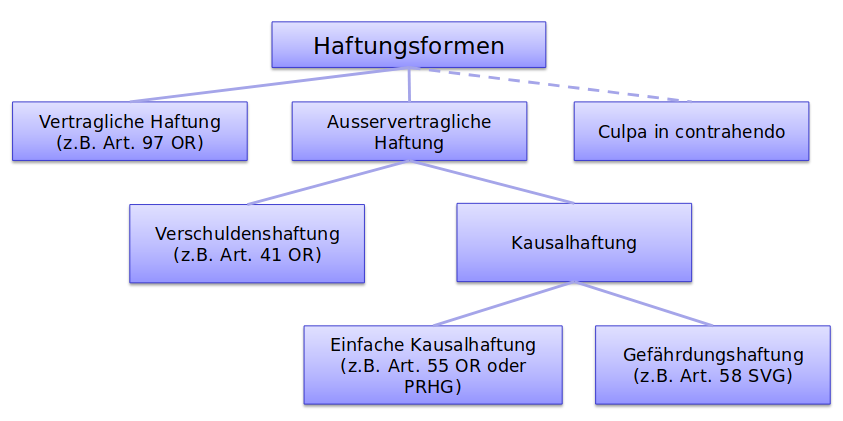
\includegraphics[width=.8\textwidth]{figures/haftpflichtrechtFormen.png}
	\caption{Formen der Haftpflicht}
\end{figure}


\subsection{Arten von ausservertraglichen Haftungen}
\label{sec:Haftpflicht-Arten}

\begin{description}
	\item[Verschuldungshaftung] Schädiger haftet grundsätzlich nur, wenn
	er den Eintritt des Schadens verschuldet hat (Persönliche
	Vorwerfbarkeit). (Art. 41 OR)
	\item[Kausalhaftung] Setzt kein Verschulden voraus, sondern ist
	gegeben, wenn durch das Gesetz festgelegte Tatbestandsvoraussetzungen
	erfüllt sind.
	\begin{itemize}
		\tightlist
		\item einfache Kausalhaftung
		\begin{itemize}
			\tightlist
			\item Geschäftsherrenhaftung (Art. 55 OR) - Chef haftet für Mitarbeiter
			\item Werkeigentümerhaftung (Art. 58 OR) - Haft für Werke (Baugerüste,
			Häuser, \ldots{})
			\item Haftung des Grundeigentümers (Art. 679 ZGB)
			\item Produktehaftpflicht (PrHG)
		\end{itemize}
		\item Gefährdungshaftung: Bestimmten Einrichtungen sind Gefahren inhärent,
		die den Betreibern dieser Einrichtungen eine besondere Verantwortung
		aufbürden (Gefahrensatz).
	\end{itemize}
\end{description}


\subsection{Voraussetzungen}

\begin{figure}[H]
	\centering
	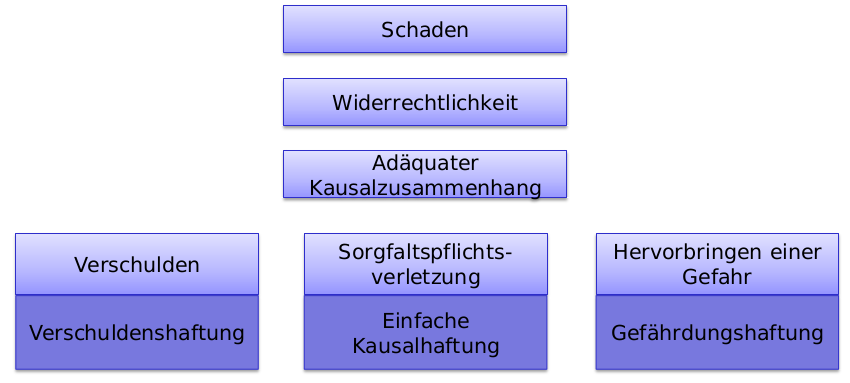
\includegraphics[width=.8\textwidth]{figures/haftpflichtVerschulden.png}
	\caption{Voraussetzungen bei Verschuldens- und Kausalhaftung}
\end{figure}

Folgende Punkte müssen \textbf{zwingend erfüllt sein}, damit eine Haftpflicht
vorliegt:

\begin{itemize}
\tightlist
\item Schaden
\item Wiederrechtlichkeit
\item Adäquater Kausalzusammenhang
\item Verschulden
\end{itemize}


\subsubsection{Definition Schaden (Vermögenseinbusse)}

Schaden ist eine unfreiwillige Verminderung des Vermögens in Form von:
\begin{itemize}
	\tightlist
	\item Abnahme der Aktiven
	\item Zunahme der Passiven
	\item Entgangener Gewinn
\end{itemize}

Der Schaden als Vermögenseinbusse bestimmt sich grundsätzlich nach
der \textbf{Differenz} zwischen dem gegenwärtigen Vermögensstand und dem Stand,
den das Vermögen ohne das schädigende Ereignis hätte.


\subsubsection{Schadensformen}

\begin{itemize}
	\tightlist
	\item Vermögensschaden (Schaden welcher weder Sach- noch Personenschaden ist)\\
	Kann nur beim vorliegen einer Schutznorm (gesetzliche Regelung) geltend
	gemacht werden.
	\item Personenschaden (Beeinträchtigung der Gesundheit einer Person)\\
	Vermögensschaden durch Heilungskosten, Lohnausfall usw.
	\item Sachschaden (Wenn eine Sache Schaden nimmt, wie z.B. ein Laptop)
	\item Immaterieller Schaden (Reputation, Persönlichkeitsverletzung)
	\item Direkter Schaden (Der Schaden ist durch das schädige Ereignis direkt
	ausgelöst)
	\item Indirekter Schaden (Der Schaden entsteht später als das schädigende
	Ereignis). Folgeschaden.
\end{itemize}


\subsubsection{Definition Wiederrechtlichkeit}

\begin{itemize}
	\tightlist
	\item Es muss entweder ein absolutes Recht verletzt sein
	\begin{itemize}
		\tightlist
		\item Absolute Rechte sind Rechte, die gegenüber allen gelten
		\begin{itemize}
			\tightlist
			\item Besitz / Eigentum
			\item Leben
			\item Ehre
			\item Gesundheit
		\end{itemize}
	\end{itemize}
	\item Oder es muss eine Schutznom verletzt werden
	\begin{itemize}
		\tightlist
		\item Veruntreuung oder Datenbeschädigung
	\end{itemize}
\end{itemize}


\paragraph{Rechtfertigungsgründe}
\label{sec:Haftpflichtrecht-Rechtfertigung}
\begin{itemize}
	\tightlist
	\item Notwehr (Art. 52.1 OR) - Verhältnismässige Abwehr in einer
	Notsituation
	\item Notstand (Art. 52.2 OR) - Um sich selber zu schützen, greift man in
	das Rechtsgut eines anderen ein.
	\item Selbsthilfe (Art. 52.3 OR) - Die eigene Sache darf wieder veschaft
	werden (ohne Selbstjustiz)
	\item Einwilligung des Verletzten - z.B. eine Operation
	\item Amtspflicht - z.B. Taschenkontrolle durch einen Polizisten
\end{itemize}

\subsubsection{Definition: Adäquater Kausalzusammenhang}

Ein Kausalzusammenhang ist adäquat, wenn die betreffende Ursache
nach dem gewöhnlichen Lauf der Dinge und der allgemeinen
Lebenserfahrung an sich geeignet war, den eingetretenen Erfolg zu
bewirken, so dass der Eintritt dieses Erfolges als durch die fragliche
Tatsache allgemein begünstigt erscheint.\\
-> Schaden ist effektiv aus der Tat hervorgegangen.


\subsubsection{Verschuldungsformen}

\begin{description}
	\item[Vorsatz] Der Schuldner strebt einen Erfolg bewusst an.
	\item[Eventualvorsatz] Der Schädiger nimmt ein Schaden in Kauf.
	\item[Fahrlässigkeit] Nicht absichtlich angestrebte
	\emph{mangelhafte Sorgfalt} führt zur Verletzung.\\
	Kriterium: Durchschnittliches Verhalten eines
	vernünftigen und ordentlichen Menschen.
	\begin{description}
		\tightlist
		\item[Grobe Fahrlässigkeit] Die gebotene Sorgfaltspflicht ist in
		besonders schwerer Weise verletzt.
		\item[Leichte Fahrlässigkeit] Das Verhalten des Schädigers kann
		als ``einigermassen verständlich'' bezeichnet werden. z.B. wenn man
		aus Versehen jemand mit einer Dampfwalze überfährt
	\end{description}
\end{description}

\subsection{Beweislast}

\begin{figure}[H]
	\centering
	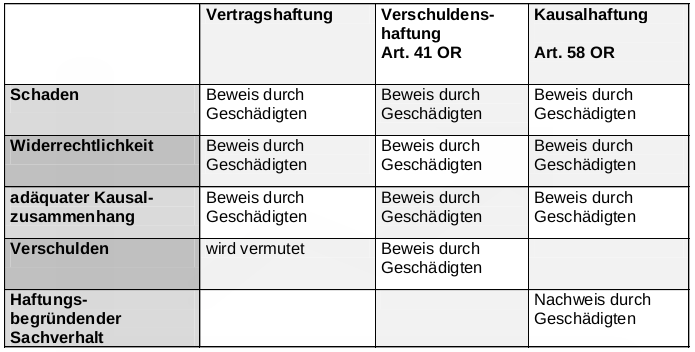
\includegraphics[width=.8\textwidth]{figures/Voraussetzungen_Haftpflichtrecht.png}
	\caption{Beweislast bei den verschiedenen Haftungstypen}
\end{figure}



\subsection{Werkeigentümerhaftpflicht}

Ihrem Unternehmen gehört eine Lokalität im Herzen der Altstadt von
Liestal. Herr X, interessiert sich für Ihre Produkte, die er im
Schaufenster sieht und möchte Ihren Laden betreten. Er rutscht auf dem
Eis vor der Ausgangstüre aus und verletzt sich am Knöchel. Liegt hier
ein Fall der Werkeigentümerhaftpflicht vor? (Art. 58 OR)

\begin{itemize}
	\tightlist
	\item Schaden: Der Knöchel ging defekt, der Arzt kostet
	\item Verschulden: Mangelhafte Unterhaltung des Werkes
	\item Wiederrechtlichkeit: Unbetrittenes Recht für Gesundheit wurde
	verletzt
	\item Werk: Alles, was künstlich hergestellt und mit dem Boden verbunden ist
	\item Vorliegen eines Werkmangels: Werk bietet bei bestimmungsgemässen
	Gebrauch keine genügende Sicherheit
	\item Kausalzusammenhang
	\item Mangelnder Unterhalt
	\item BGer: ``Wer den Besuchern eines Verkaufslokals eine Ausgangstüre zur
	Verfügung stellt, hat für deren möglichst gefahrlose Benützbarkeit zu
	sorgen. Dazu gehört auch, dass er unmittelbar jenseits der Türe
	laufende Gefahren, wie Glatteis auf dem Trottoir, im Rahmen des
	Möglichen und Zumutbaren beseitigt oder zumindest mit einem Warnschild
	(Achtung gschliferig) darauf aufmerksam macht.''
\end{itemize}

\subsection{Produktehaftpflichtgesetz}

\begin{figure}[H]
	\centering
	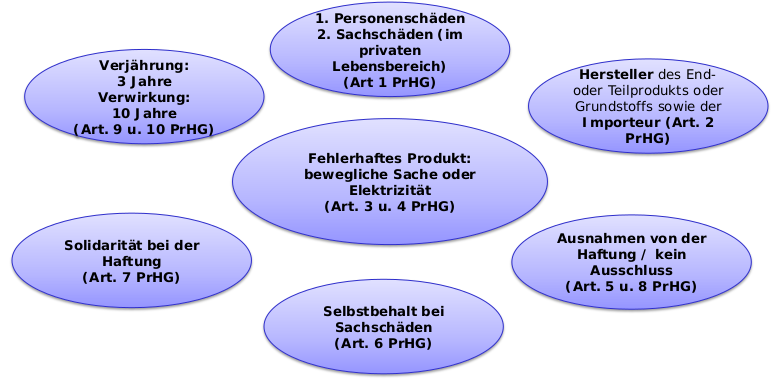
\includegraphics[width=.8\textwidth]{figures/produkthaftpflicht.png}
	\caption{Privathaftpflichtgesetz}
\end{figure}

\begin{itemize}
	\tightlist
	\item Der Schaden an Personen ist gedeckt
	\item Private Sachschäden sind auch gedeckt. Werden jedoch Dinge von einem
	Unternehmen beschädigt, ist dies nicht gedeckt.
	\item Produkthaftpflicht darf nicht durch AGBs oder andere Verträge
	ausgeschlossen werden
	\item Solidarität bei der Haftung heisst: Auch wenn man als Importeur z.B.
	nichts für das Versagen des Produkts hat, haftet man und muss zahlen.
	\item Die Produktehaftpflicht gilt nur 10 Jahre nach Einführung des Produkts
	und 3 Jahre nach Eintritt eines Schadens
\end{itemize}

\subsection{Gefährdungshaftung}
\label{sec:Haftpflicht-Gefaerdungshaftung}
Die Gefährdungshaftung ist eine qualifizierte Kausalhaftung, indem sie
davon ausgeht, dass bestimmten Einrichtungen Gefahren inhärent sind, die
den Betreibern dieser Einrichtungen eine besondere Verantwortung
aufbürden.\\
BSP: Haftpflicht des Motorfahrzeughalters (SVG)

\paragraph{Art. 58.1 SVG}
Wird durch den Betrieb eines Motorfahrzeuges ein Mensch getötet oder
verletzt oder Sachschaden verursacht, so haftet der Halter für den
Schaden.


\subsection{Culpa in contrahendo}

Ist im Gesetz nirgends geregelt.

„Verschulden bei Vertragsverhandlung`` Voraussetzungen:

\begin{itemize}
	\tightlist
	\item es werden Verhandlungen über einen zukünftigen Vertrag geführt,
	\item vorvertragliche Pflichten werden verletzt,
	\item eine der Vertragsparteien erleidet einen Schaden, welcher
	\item adäquat-kausal aus der Pflichtverletzung hervorgeht
	\item und dem Verschulden der schädigenden Person zuzuschreiben ist.
\end{itemize}

    \section{Öffentlichkeitsprinzip und Open Data}

Compliance für die öffentliche Verwaltung erfordert:

\begin{itemize}
	\tightlist
	\item Transparenz
	\item Nachvollziehbarkeit
	\item 4-Augen-Prinzip
\end{itemize}

Diese Anforderungen haben zum \textbf{Öffentlichkeitsgesetz (BGÖ)} und der
\textbf{elektronischen Geschäftsverwaltung (GEVER)} geführt.

\subsection{Inhalt des BGÖ}
Alle Personen erhalten danach grundsätzlich Zugang zu jeder Information und
jedem Dokument der Bundesverwaltung. Dies gilt jedoch nicht, wenn
insbesondere die Privatsphäre Dritter verletzt oder die Sicherheit der Schweiz
gefährdet werden kann.\\
In der Schweiz ist dieses Gesetz am 1. Juli 2006 inkraftgetreten.\\

Die meisten Kantone haben selbst auch ein solches Gesetz auf kantonaler Ebene.
Kein solches Gesetz haben aktuell noch die Kantone Thurgau (in Diskussion),
Appenzell Ausserrhoden, Glarus (in Diskussion), Luzern, Obwalden und Nidwalden.\\

Dies ist ein grosser Paradigmenwechsel, denn früher galt:\\
Alle Informationen waren geheim (mit Ausnahmen), kein Anspruch auf Information
über die Verwaltungstätigkeit, kein Anspruch auf Dokumentenzugang,
freies Ermessen der Behörden bei der Gewährung von Ausnahmen.

\subsection{Ziele des BGÖ}

\begin{itemize}
	\tightlist
	\item Kultur der Transparenz in der Verwaltung – Informationsbedürfnisse
	berücksichtigen
	\item Durchsetzbares Recht auf Zugang zu amtlichen Dokumenten für jede
	Person (kein besonderes Interesse muss nachgewiesen werden)
	\item Verbesserung Beziehung Staat und Bürger
	\item Stärkung demokratischer Kontrollrechte
	\item Information als Voraussetzung für politische Mitwirkung
	\item Effizienzgewinn in der Verwaltung
	\item Vorteile für die Wirtschaft
\end{itemize}

\subsection{Geltungsbereich des BGÖ}

Das Gesetz gilt gemäss Art. 5 des BGÖ für \textbf{Amtliche Dokumente, die nach
Inkrafttreten des BGÖ entstanden sind:}
\begin{itemize}
	\tightlist
	\item Information auf beliebigem Informationsträger
	\item Information im Besitz einer Behörde
	\item Zur Erfüllung einer öffentlichen Aufgabe
\end{itemize}

Ausgenommen sind dabei:
\begin{itemize}
	\tightlist
	\item Kommerziell genutzte Dokumente (Geodaten)
	\item Nicht fertiggestellte Dokumente (Entwürfe)
	\item Dokumente für persönlichen Gebrauch (Notizen)
\end{itemize}

Als \textbf{amtliche Dokumente} gelten alle Dokumente welche von der
\textit{Bundesverwaltung}, \textit{Organisationen und Personen des öffentlichen
und privaten Rechts (Post, SBB, SUCA etc.)} und \textit{Parlamentsdienste}
veröffentlicht werden. Es gilt nicht für die \textit{Schweizerische Nationalbank}
sowie die \textit{Eidgenössische Finanzmarktaufsicht} (Art.2 BGÖ).

\subsubsection{Ausnahmen (Art. 7 BGÖ)}
\textbf{Zugang wird eingeschränkt, aufgeschoben oder verweigert:}
\begin{itemize}
	\tightlist
	\item Freie Meinungs- und Willensbildung einer Behörde
	\item Durchführung behördlicher Massnahmen
	\item Innere oder äussere Sicherheit der Schweiz
	\item Aussenpolitische Interessen oder die internationalen Beziehungen
	\item Beziehungen zwischen dem Bund und den Kantonen oder zwischen Kantonen
	\item Wirtschafts-, geld- und währungspolitischen Interessen der Schweiz
	\item Berufs-, Geschäfts- oder Fabrikationsgeheimnisse
	\item Informationen von Dritten freiwillig mitgeteilt.
\end{itemize}

\subsubsection{Interessenabwägung (Art. 6 BGÖ)}
Interessenabwägung zwischen dem Schutz der Privatsphären Dritter und
öffentlichem Interesse am Zugang.

\textbf{Das öffentliche Interesse kann überwiegen:}
\begin{itemize}
	\tightlist
	\item Beim Vorliegen eines besonderen Informationsinteresses der Öffentlichkeit
	(z.B. Korruptionsvorfälle)
	\item Beim Schutz spezifischer öffentlicher Interessen wie öffentliche Ordnung
	und	Sicherheit oder öffentliche Gesundheit
	\item Bei Empfängern von Finanzhilfen oder Abgeltungen
\end{itemize}

\subsection{OpenData}
Offene Daten sind sämtliche Datenbestände, die im Interesse der Allgemeinheit
der Gesellschaft ohne jedwede Einschränkung zur freien Nutzung, zur
Weiterverbreitung und zur freien Weiterverwendung frei zugänglich gemacht
werden.\\

Der Staat hat für die Bürger die Infrastruktur bereit zu stellen. Dazu
gehören zunehmend auch Daten. Dies bietet eingrosses Potential für neue Produkte
\& Dienstleistungen. Grundlage für zahlreiche AI-Anwendungen (als Testdaten,
als Grundlage für Anwendungen).

\subsubsection{OpenData und digitale Transformation}

\begin{itemize}
	\tightlist
	\item opendata.swiss ist das Portal des Bundes \& einiger (weniger) Kantone und
	Gemeinden für öffentlich zugängliche Daten.
	\item Teil der Open-Government-Data-Strategie Schweiz 2014-2018 des
	Bundesrates (e-Government). Bundesrat verabschiedet in den nächsten
	Wochen die Fortsetzung und veröffentlicht Bericht.
	\item Einige Datensätze sind frei verfügbar und dürfen auch kommerziell genutzt
	werden, andere nur mit Einwilligung und Gebühr.
	\item Eher Zurückhaltung der Kantone (Ausnahme z.B. OpenZH) und Gemeinden, da
	man mit den Daten vielleicht Geld verdienen könnte. Kurzfristige Sichtweise.
\end{itemize}
    \hypertarget{grundzuxfcge-des-haftpflichtrechtes-gemuxe4ss-or-und-spezialgesetzen}{%
\section{Grundzüge des Haftpflichtrechtes gemäss OR und
Spezialgesetzen}\label{grundzuxfcge-des-haftpflichtrechtes-gemuxe4ss-or-und-spezialgesetzen}}

\hypertarget{werkeigentuxfcmerhaftpflicht}{%
\subsection{Werkeigentümerhaftpflicht}\label{werkeigentuxfcmerhaftpflicht}}

Ihrem Unternehmen gehört eine Lokalität im Herzen der Altstadt von
Liestal. Herr X, interessiert sich für Ihre Produkte, die er im
Schaufenster sieht und möchte Ihren Laden betreten. Er rutscht auf dem
Eis vor der Ausgangstüre aus und verletzt sich am Knöchel. Liegt hier
ein Fall der Werkeigentümerhaftpflicht vor? (Art. 58 OR)

\begin{itemize}
\tightlist
\item
  Schaden - Der Knöchel ging defekt, der Arzt kostet
\item
  Verschulden - Mangelhafte Unterhaltung des Werkes
\item
  Wiederrechtlichkeit - Unbetrittenes Recht für Gesundheit wurde
  verletzt
\item
  Werk: Alles, was künstlich hergestellt und mit dem Boden verbunden ist
\item
  Vorliegen eines Werkmangels: Werk bietet bei bestimmungsgemässen
  Gebrauch keine genügende Sicherheit
\item
  Kausalzusammenhang
\item
  Mangelnder Unterhalt
\item
  BGer: ``Wer den Besuchern eines Verkaufslokals eine Ausgangstüre zur
  Verfügung stellt, hat für deren möglichst gefahrlose Benützbarkeit zu
  sorgen. Dazu gehört auch, dass er unmittelbar jenseits der Türe
  laufende Gefahren, wie Glatteis auf dem Trottoir, im Rahmen des
  Möglichen und Zumutbaren beseitigt oder zumindest mit einem Warnschild
  (Achtung gschliferig) darauf aufmerksam macht.''
\end{itemize}

\hypertarget{produktehaftpflichtgesetz}{%
\subsection{Produktehaftpflichtgesetz}\label{produktehaftpflichtgesetz}}

\begin{figure}
\centering
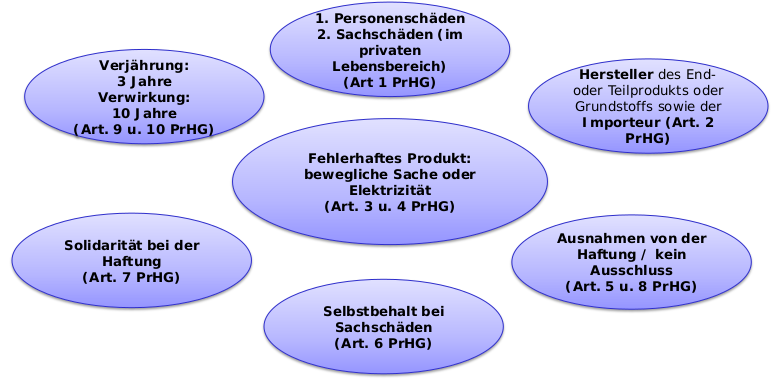
\includegraphics{figures/produkthaftpflicht.png}
\caption{Privathaftpflichtgesetz}
\end{figure}

\begin{itemize}
\tightlist
\item
  Der Schaden an Personen ist gedeckt
\item
  Private Sachschäden sind auch gedeckt. Werden jedoch Dinge von einem
  Unternehmen beschädigt, ist dies nicht gedeckt.
\item
  Produkthaftpflicht darf nicht durch AGBs oder andere Verträge
  ausgeschlossen werden
\item
  Solidarität bei der Haftung heisst: Auch wenn man als Importeur z.B.
  nichts für das Versagen des Produkts hat, haftet man und muss zahlen.
\item
  Die Produktehaftpflicht gilt nur 10 Jahre nach Einführung des Produkts
  und 3 Jahre nach Eintritt eines Schadens
\end{itemize}

\hypertarget{gefuxe4hrdungshaftung}{%
\subsection{Gefährdungshaftung}\label{gefuxe4hrdungshaftung}}

Die Gefährdungshaftung ist eine qualifizierte Kausalhaftung, indem sie
davon ausgeht, dass bestimmten Einrichtungen Gefahren inhärent sind, die
den Betreibern dieser Einrichtungen eine besondere Verantwortung
aufbürden.\\
BSP: Haftpflicht des Motorfahrzeughalters (SVG)

Art. 58.1 SVG

\begin{itemize}
\tightlist
\item
  Wird durch den Betrieb eines Motorfahrzeuges ein Mensch getötet oder
  verletzt oder Sachschaden verursacht, so haftet der Halter für den
  Schaden.
\end{itemize}

\hypertarget{voraussetzungen-haftpflichtrecht}{%
\subsection{Voraussetzungen
Haftpflichtrecht}\label{voraussetzungen-haftpflichtrecht}}

\begin{figure}
\centering
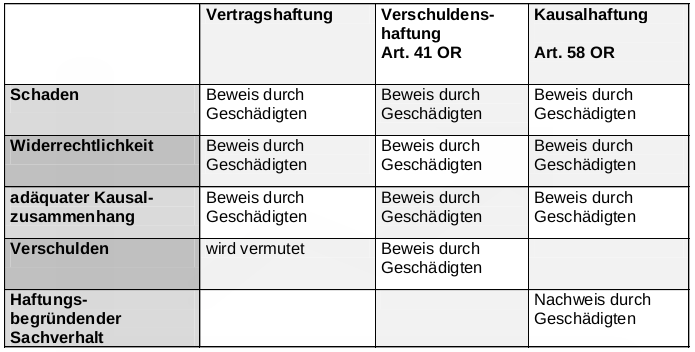
\includegraphics{figures/Voraussetzungen_Haftpflichtrecht.png}
\caption{Voraussetzungen Haftpflichtrecht}
\end{figure}

\hypertarget{culpa-in-contrahendo}{%
\subsection{Culpa in contrahendo}\label{culpa-in-contrahendo}}

Ist im Gesetz nirgends geregelt.

„Verschulden bei Vertragsverhandlung`` Voraussetzungen:

\begin{itemize}
\tightlist
\item
  es werden Verhandlungen über einen zukünftigen Vertrag geführt,
\item
  vorvertragliche Pflichten werden verletzt,
\item
  eine der Vertragsparteien erleidet einen Schaden, welcher
\item
  adäquat-kausal aus der Pflichtverletzung hervorgeht
\item
  und dem Verschulden der schädigenden Person zuzuschreiben ist.
\end{itemize}

\end{document}